\documentclass[hyperref=colorlinks]{beamer}
\mode<presentation>
\usetheme{iclpt}
\setbeamertemplate{navigation symbols}{}
\setbeamertemplate{headline}{
  \begin{beamercolorbox}[leftskip=.2cm,rightskip=.2cm,topskip=.2cm,ht=1.1cm,dp=0.1cm,wd=\textwidth]{institute in head/foot}
    
\includegraphics[height=1cm]{icl.pdf}
    \hfill
%    \includegraphics[height=1cm]{../Pics/ATLAS-Logo-Square-Blue-RGB.png}
%    
\includegraphics[height=1cm]{../Pics/CMS-Color.pdf}
    
\includegraphics[height=1cm]{TalkPics/t2k_logo_large.png}

%??put t2k logo here
  \end{beamercolorbox}
}
\setbeamertemplate{footline}{
  \begin{beamercolorbox}[ht=.35cm,dp=0.2cm,wd=\textwidth,leftskip=.3cm]{author in head/foot}%
    \begin{minipage}[c]{5cm}%
      \usebeamerfont{author in head/foot}
      \insertshortauthor 
      \insertshorttitle
    \end{minipage}\hfill%
    \hfill
    \insertframenumber{} / \ref{lastframe}
    %\hfill
    \begin{minipage}{6cm}
      \hfill
      %\insertshorttitle
    \end{minipage}
  \end{beamercolorbox}%
}

\definecolor{beamer@icdarkblue}{RGB}{0,51,102}
\definecolor{beamer@icmiddleblue}{RGB}{0,82,150} 
\definecolor{beamer@iclightblue}{RGB}{200,212,232}
\definecolor{beamer@icmiddlered}{RGB}{204,51,0}
\definecolor{beamer@iclightred}{RGB}{232,212,32}

\usepackage{tikz}
\usetikzlibrary{arrows,shapes,backgrounds}
\usepackage{color}
\usepackage{tabularx,colortbl}
\usepackage{graphicx}
\usepackage{pdfpages}
\usepackage{feynmp}
\usepackage{rotating}
\usepackage{moresize}
\usepackage{slashed}
\usepackage{xcolor,colortbl}
\DeclareGraphicsRule{*}{mps}{*}{}
\hypersetup{colorlinks=false}

\title[MaCh3 2D binning]{\vspace{-0.2cm} MaCh3 2D binning}
\author[P. Dunne]{Patrick Dunne - Imperial College London}
\titlegraphic{
  \vspace{-0.4cm}
}
\date{}
\begin{document}
\tikzstyle{every picture}+=[remember picture]
\tikzstyle{na} = [baseline=-.5ex]
\begin{fmffile}{t2ktemplatefeyndiags}


  %TITLE PAGE
  %20 mins + 5 questions
  \section{Title}
  \begin{frame}
    \titlepage
  \end{frame}

  \begin{frame}
    \frametitle{Overview}
    \begin{block}{}
        \scriptsize
        \begin{itemize}
        \item For 2016 analysis Valor and p-theta used 2D event binning in $p/E_{rec}$ and $\theta$ for $\nu_{e}$ while MaCh3 used 1D binning in $E_{rec}$
        \item We are looking to move to 2D for future analyses to make us more sensitive to differences between Asimov and observation
        \item[-] Run 6 and Run 7 data have differences in the $\theta$ distribution observed and expected
        \item[-] MaCh3 is not currently sensitive to this
        \item For now $\nu_{\mu}$ sample will still use 1D $E_{rec}$ bins, as in other analyses, but we hope to change to 2D there as well eventually.
        \item Valor splines used for $\nu_{e}$
        \item Previously showed good agreement of Asimov rates, spectra and contours from 2D with those from Valor
        \item[-] Also showed only small differences with MaCh3 1D (see backup)
        \item Will show Run 1-7c data fit comparisons today
      \end{itemize}
    \end{block}
  \end{frame}

  \begin{frame}
    \frametitle{Binning}
    \begin{block}{}
      \begin{itemize}
      \item For all studies shown today $\nu_{\mu}$ is binned in $E_{rec}$ only with 73 bins as described in TN 269
      \item For 1D TN269 MaCh3 analysis $\nu_{e}$ has 25 $E_{rec}$ bins of 50 MeV from 0 to 1.25 GeV
      \item For 2D MaCh3 analysis $\nu_{e}$ $E_{rec}$ binning is the same, but there are also 15 bins in $\theta$
      \item[-] 14 10$^\circ$ bins from 0-140$^{\circ}$ and 1 bin from 140$^{\circ}$ to 180$^{\circ}$
      \item[-] Same as Valor analysis
      \end{itemize}
    \end{block}
  \end{frame}

  \begin{frame}
    \centering
    \huge\textcolor{beamer@icmiddleblue}{Data Spectra}
  \end{frame}

  \begin{frame}
    \frametitle{$\nu_{e}$ and $\bar{\nu}_{e}$ spectra}
    \begin{columns}
      \column{.58\textwidth}
      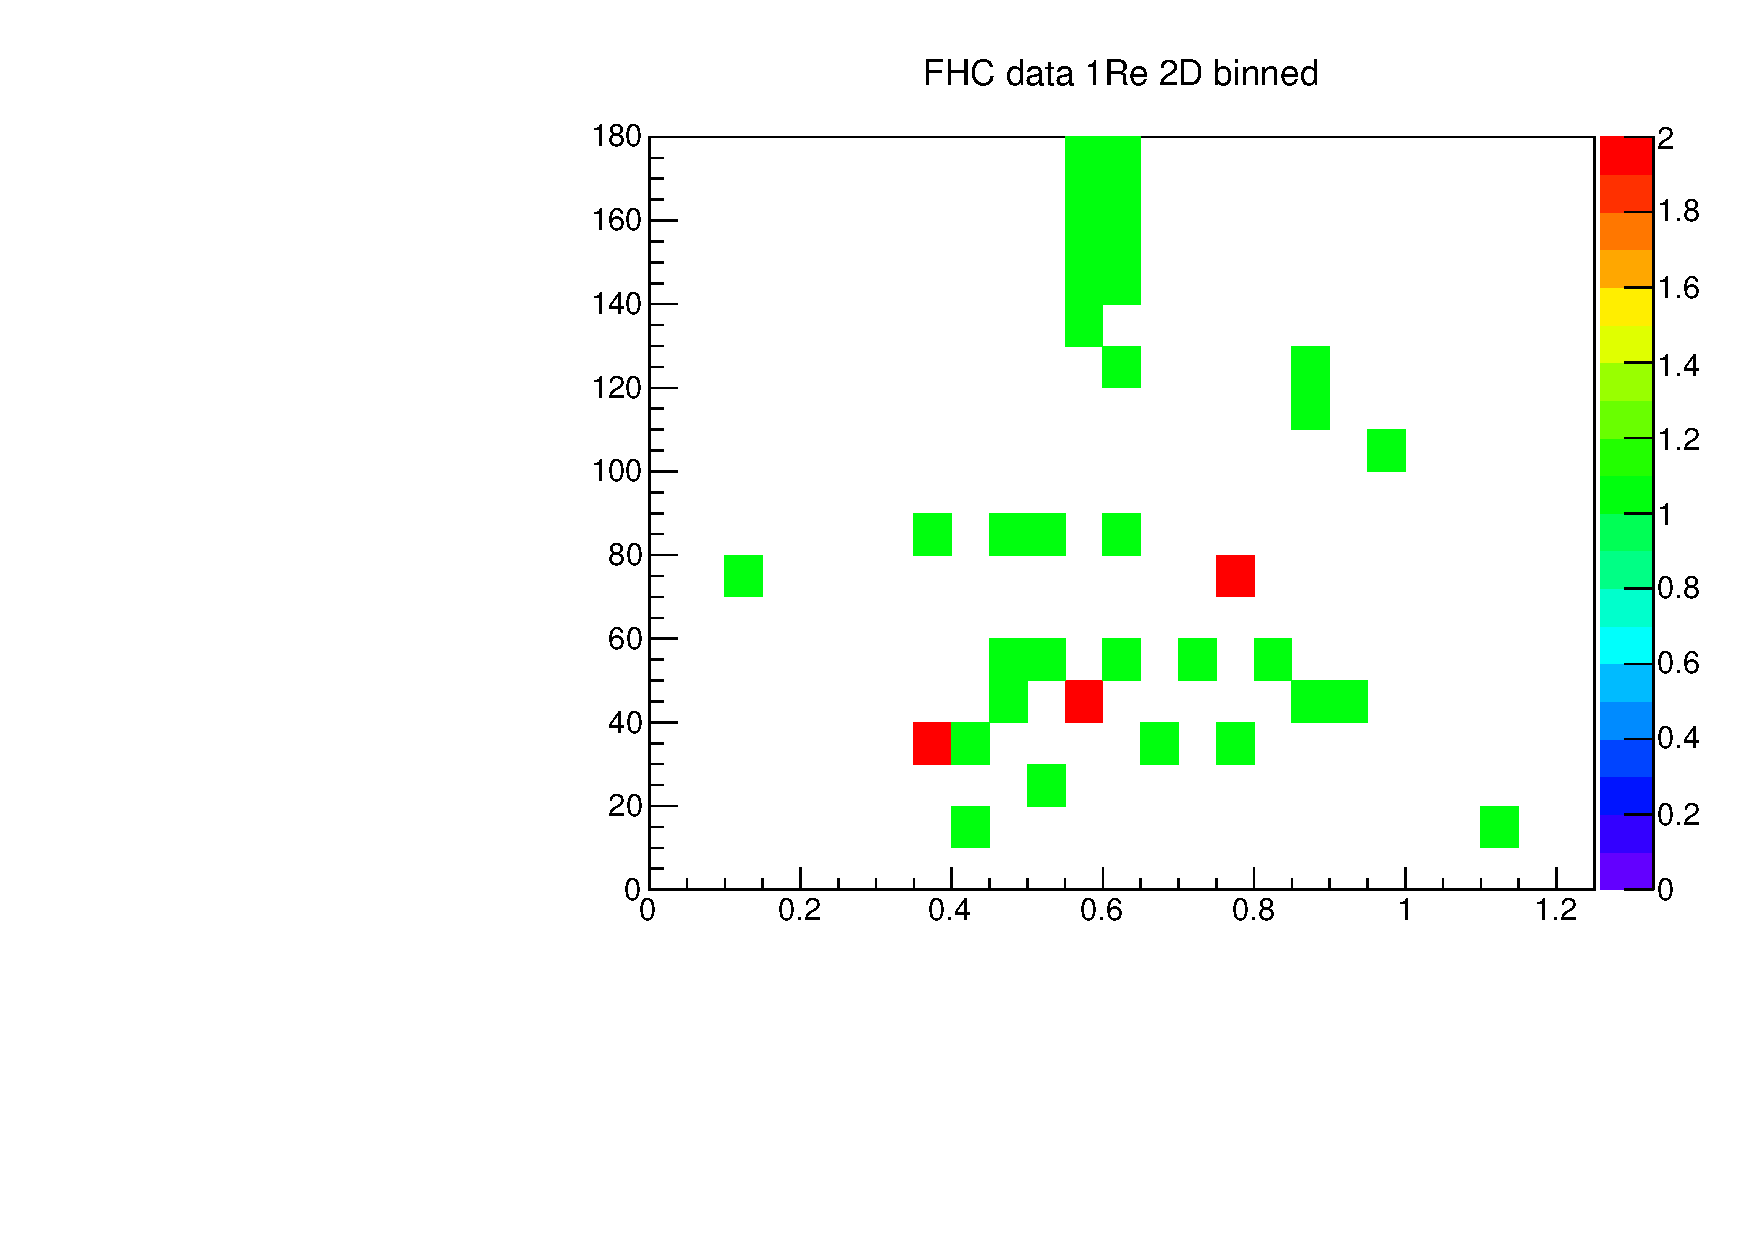
\includegraphics[width=\textwidth]{TalkPics/2Ddatafit_200916/nue_2D.pdf}
      \column{.58\textwidth}
      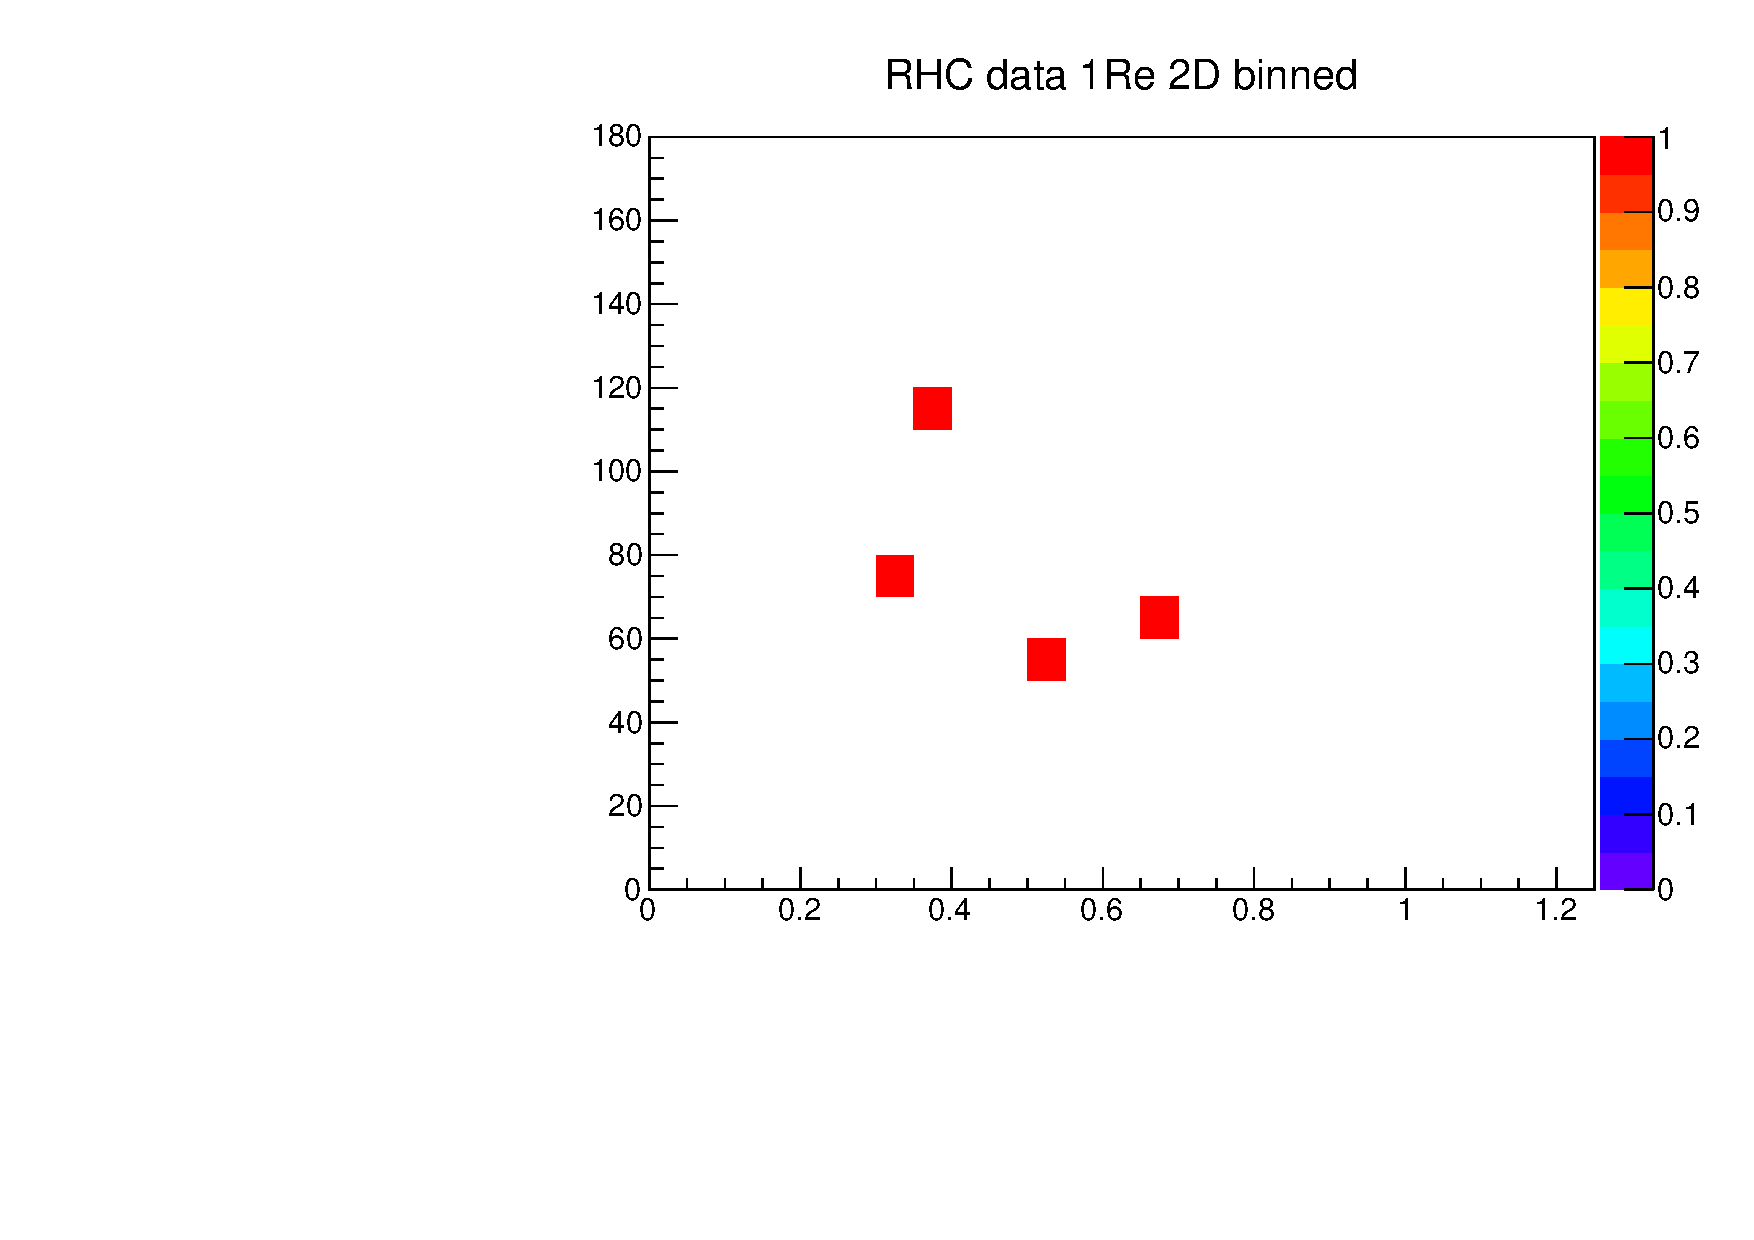
\includegraphics[width=\textwidth]{TalkPics/2Ddatafit_200916/nuebar_2D.pdf}
    \end{columns}
  \end{frame}

  \begin{frame}
    \centering
    \huge\textcolor{beamer@icmiddleblue}{MaCh3 1D-2D comparisons woRC}
  \end{frame}

  \begin{frame}
    \centering
    \begin{columns}
      \column{.6\textwidth}
      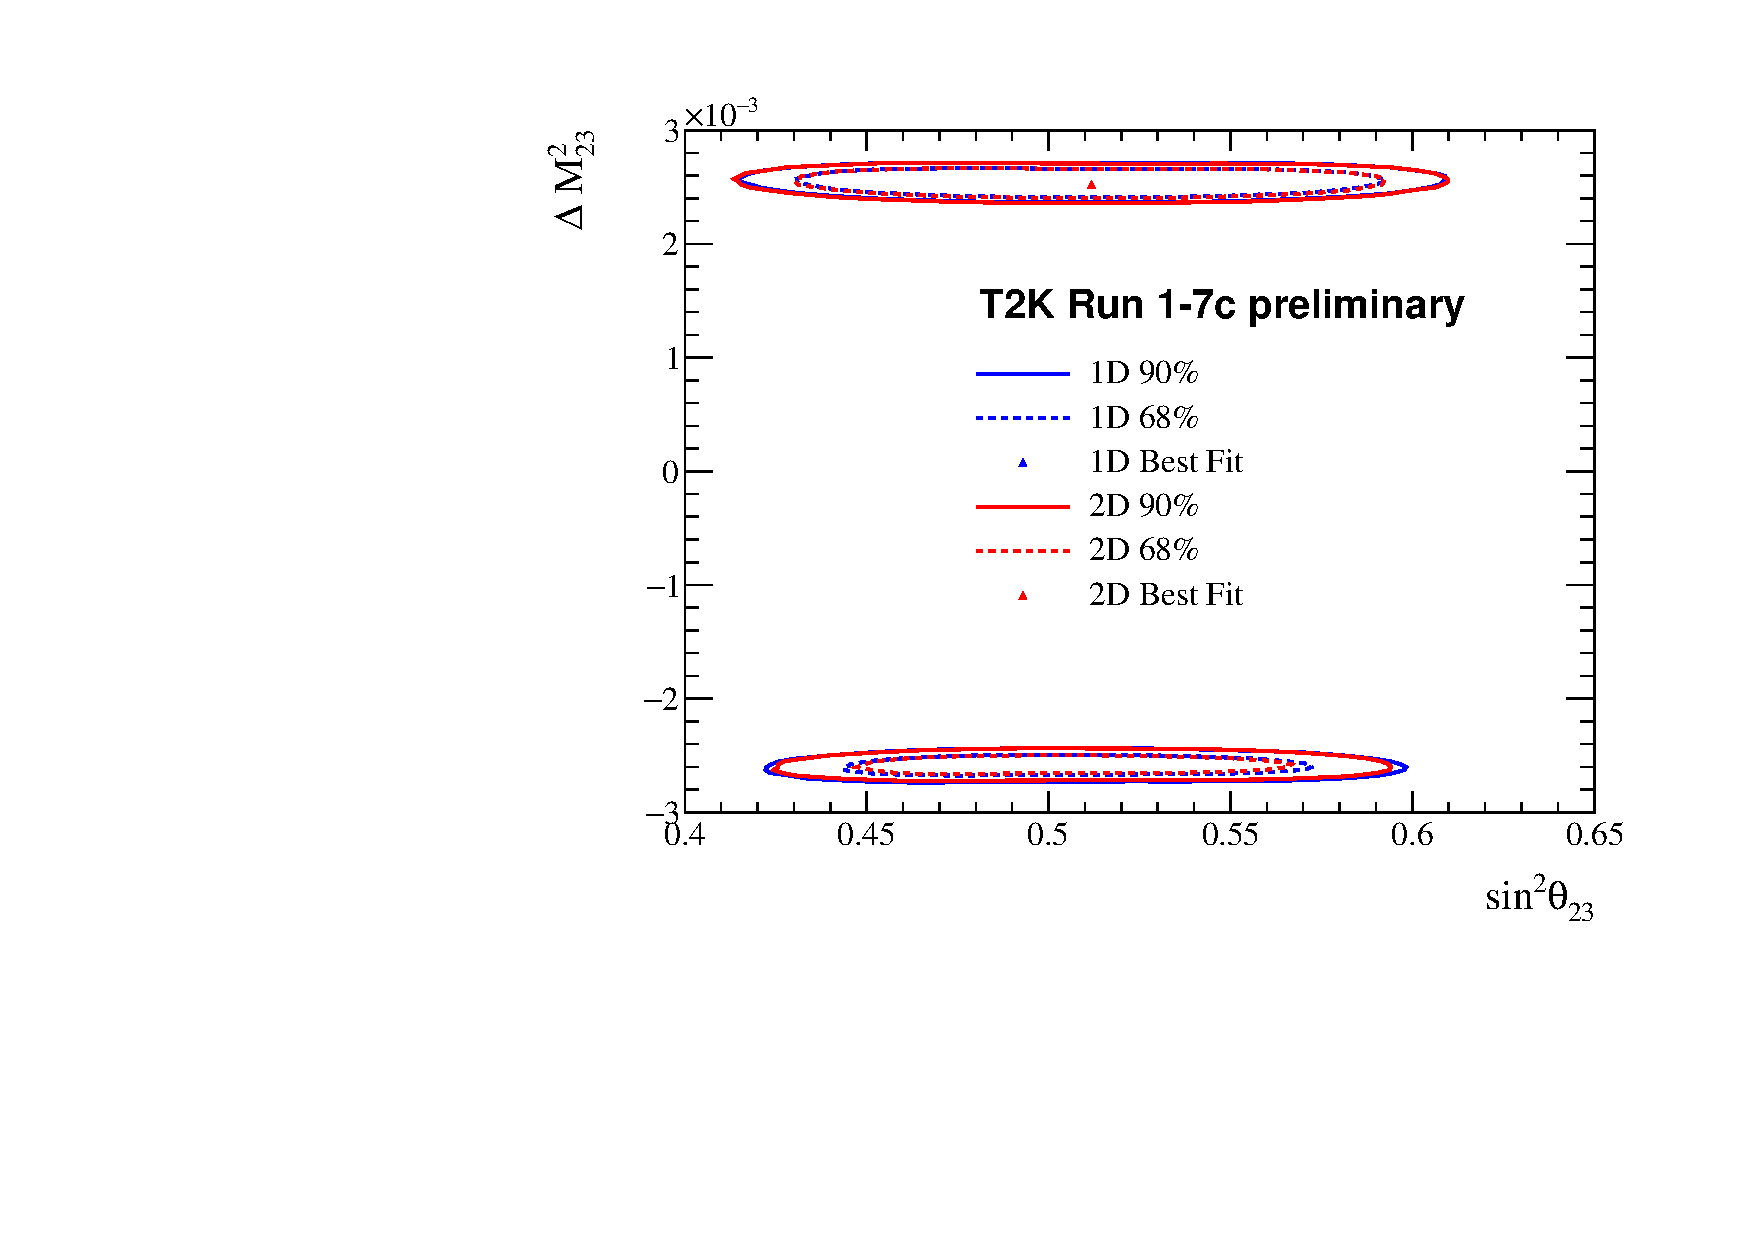
\includegraphics[width=\textwidth]{TalkPics/2Ddatafit_270916/contours_1D2Dcomparisons_woRC/comparedcontours_th23dm23_1Dvs2D_official.pdf}
      \column{.6\textwidth}
      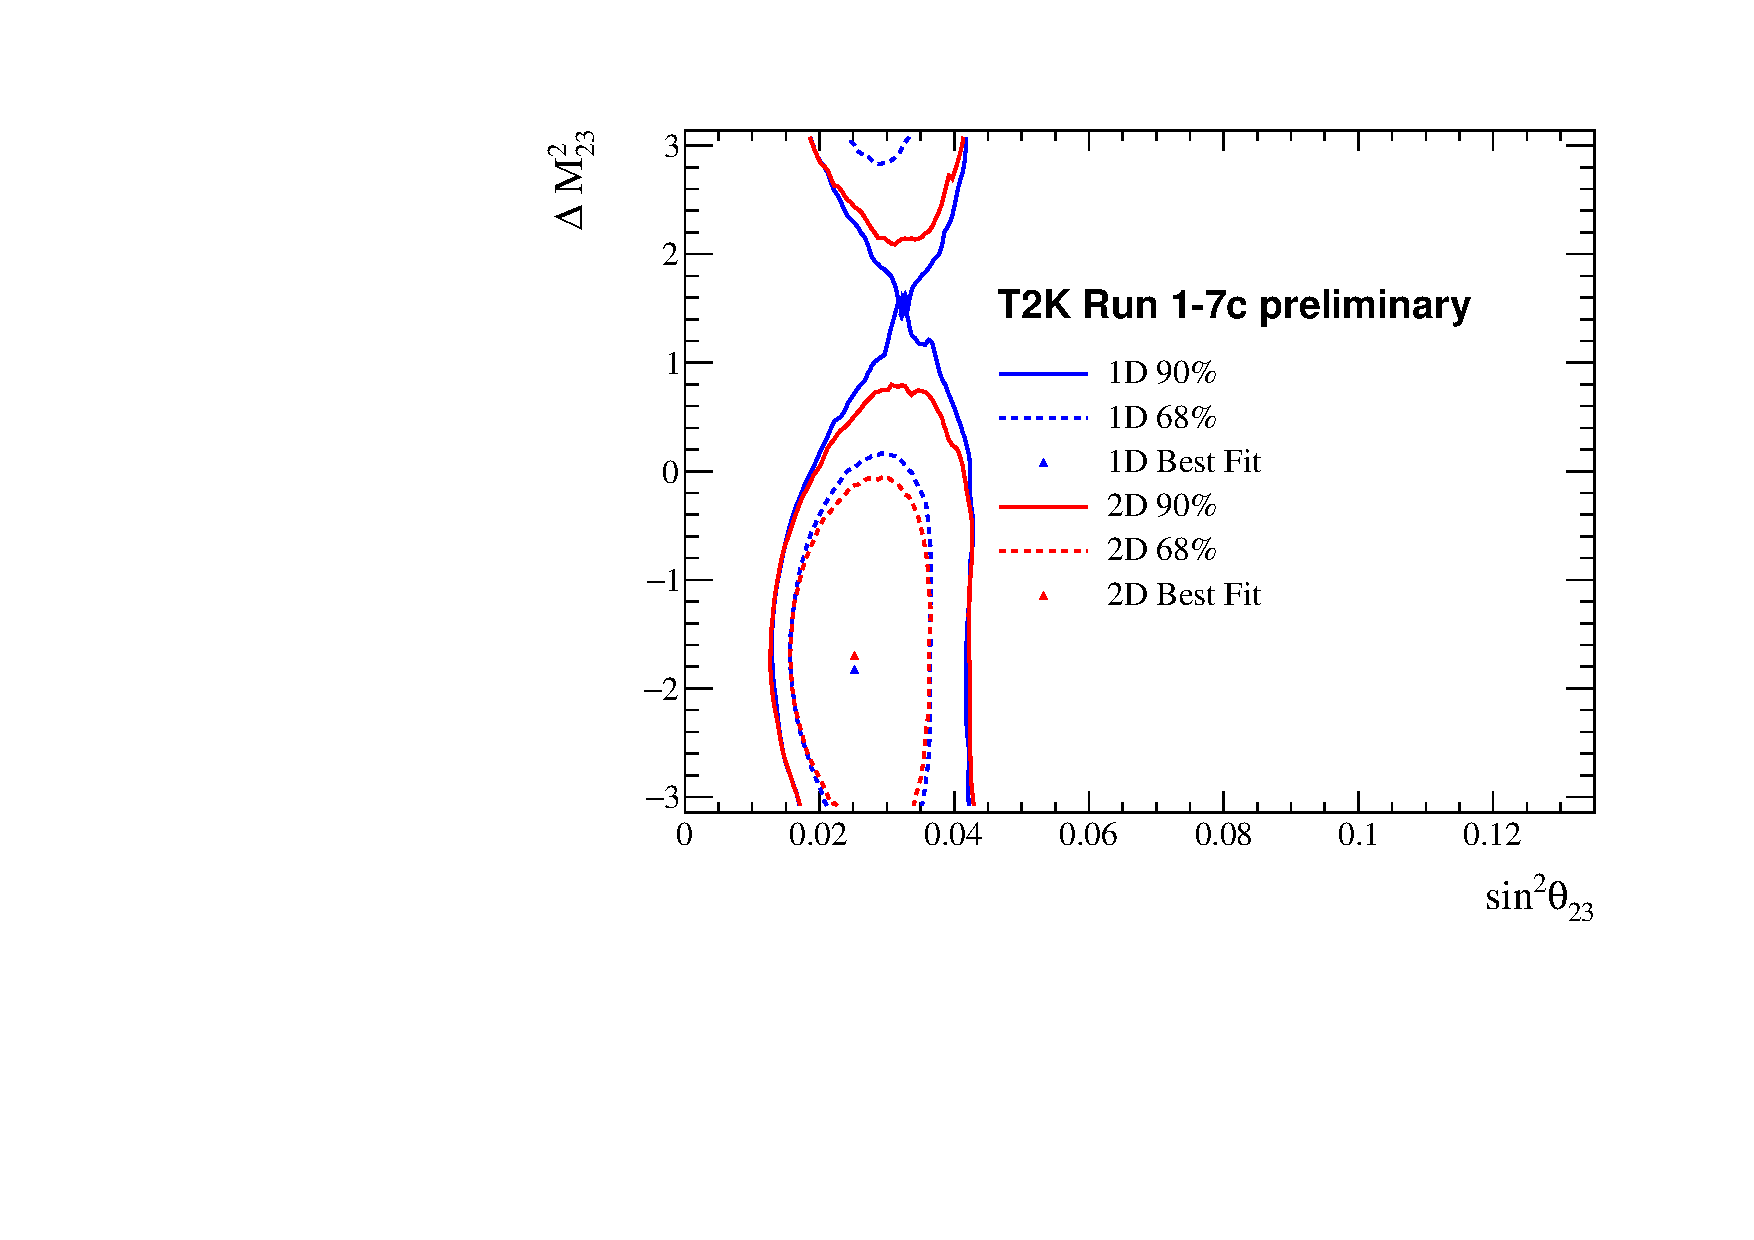
\includegraphics[width=\textwidth]{TalkPics/2Ddatafit_270916/contours_1D2Dcomparisons_woRC/comparedcontours_th13dcp_1Dvs2D_official.pdf}
    \end{columns}
  \end{frame}

  \begin{frame}
    \centering
    \begin{columns}
      \column{.6\textwidth}
      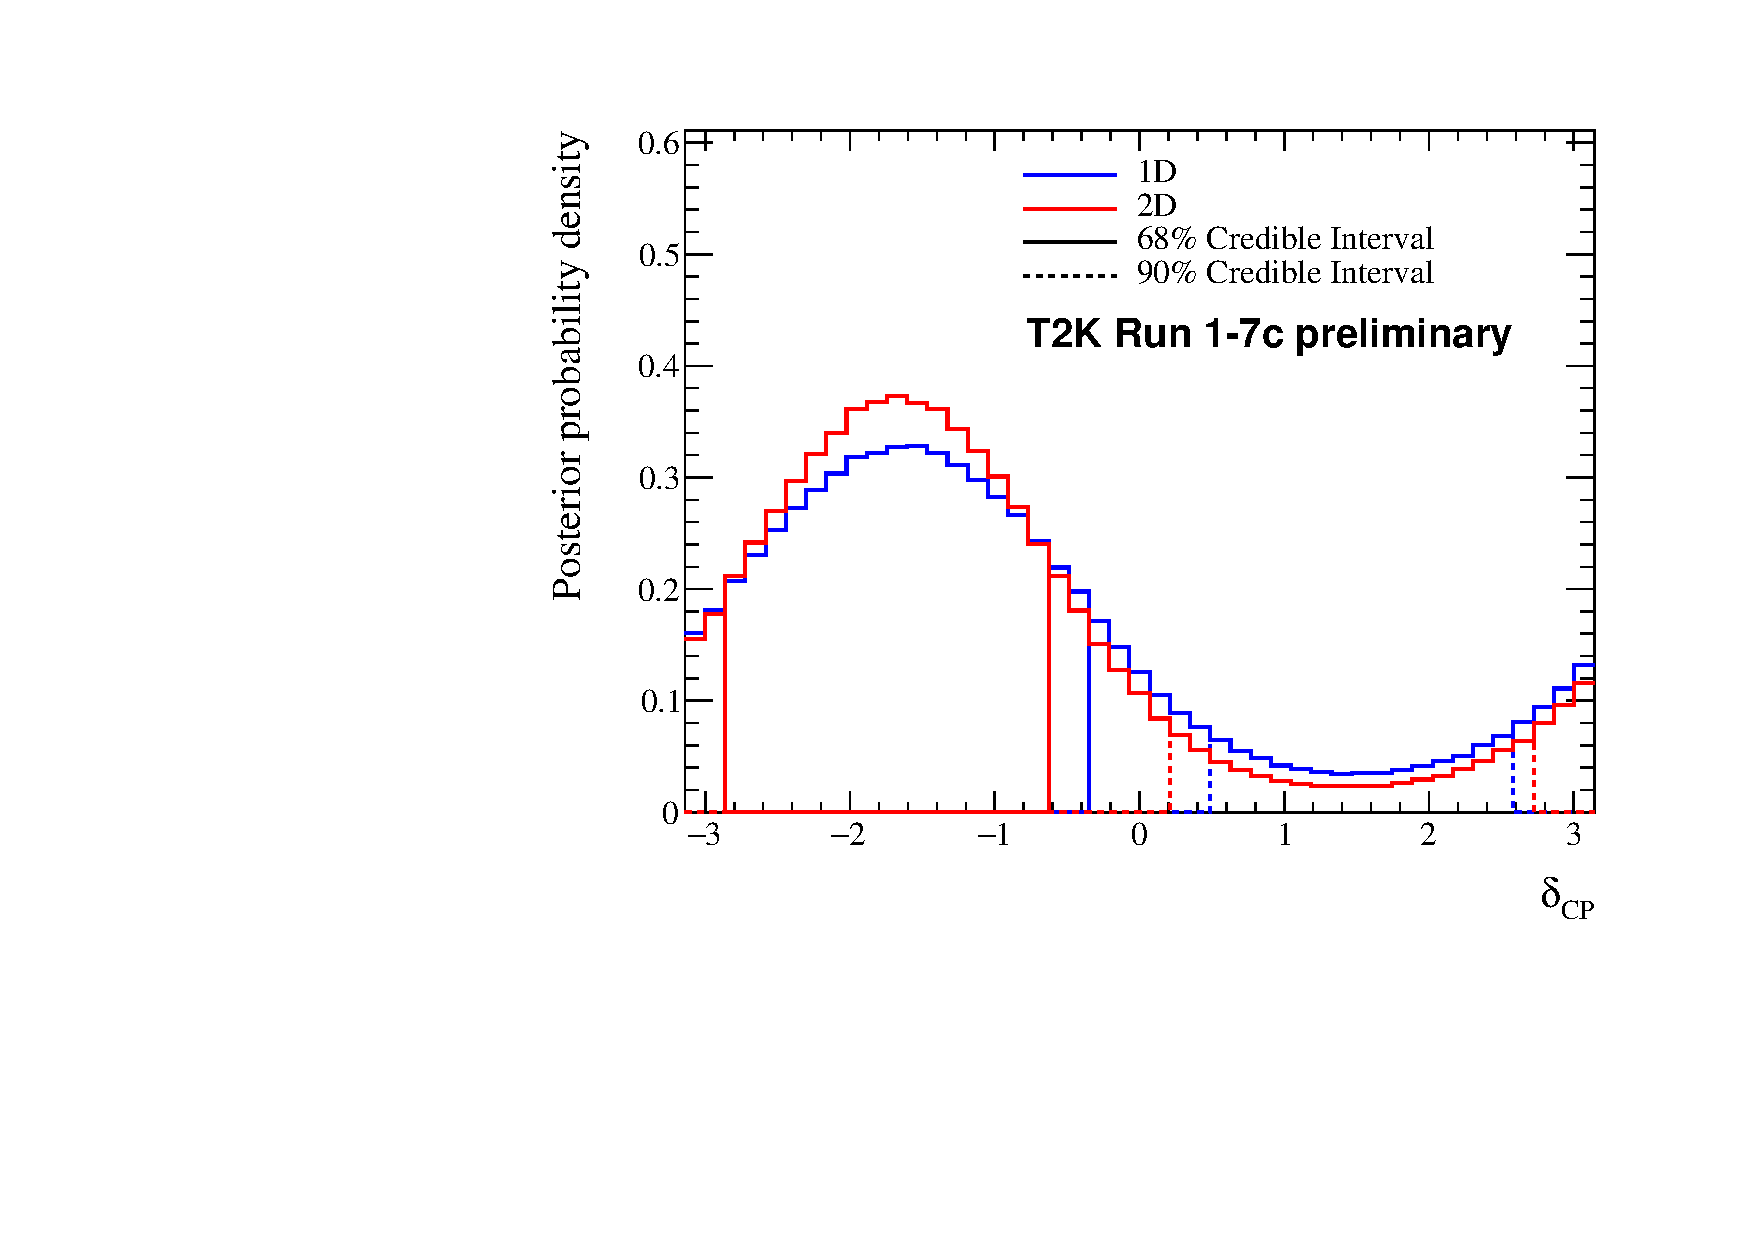
\includegraphics[width=\textwidth]{TalkPics/2Ddatafit_270916/contours_1D2Dcomparisons_woRC/contours_1D_dcp_compare_official.pdf}
    \end{columns}
  \end{frame}

  \begin{frame}
    \centering
    \huge\textcolor{beamer@icmiddleblue}{MaCh3 1D-2D comparisons wRC}
  \end{frame}

  \begin{frame}
    \centering
    \begin{columns}
      \column{.6\textwidth}
      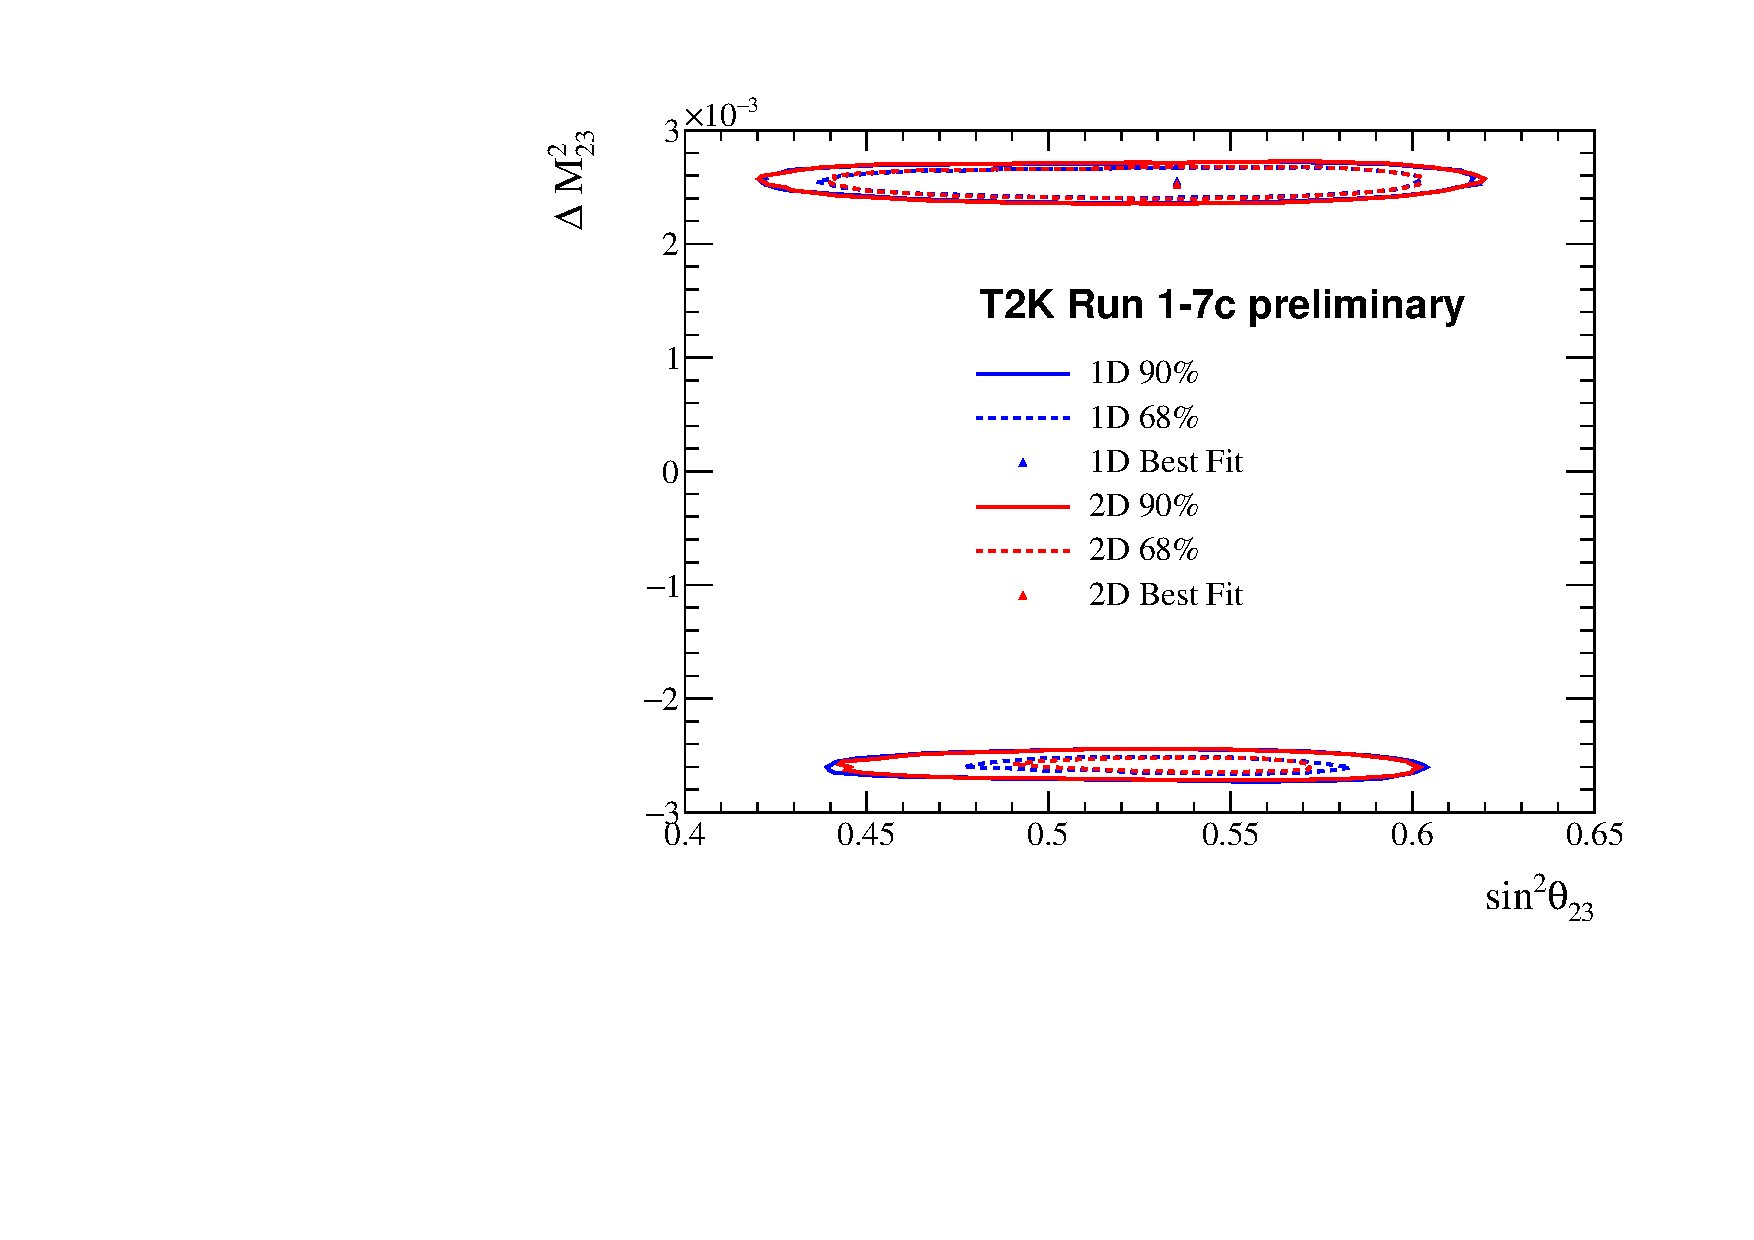
\includegraphics[width=\textwidth]{TalkPics/2Ddatafit_270916/contours_1D2Dcomparisons_wRC/comparedcontours_th23dm23_1Dvs2D_official.pdf}
      \column{.6\textwidth}
      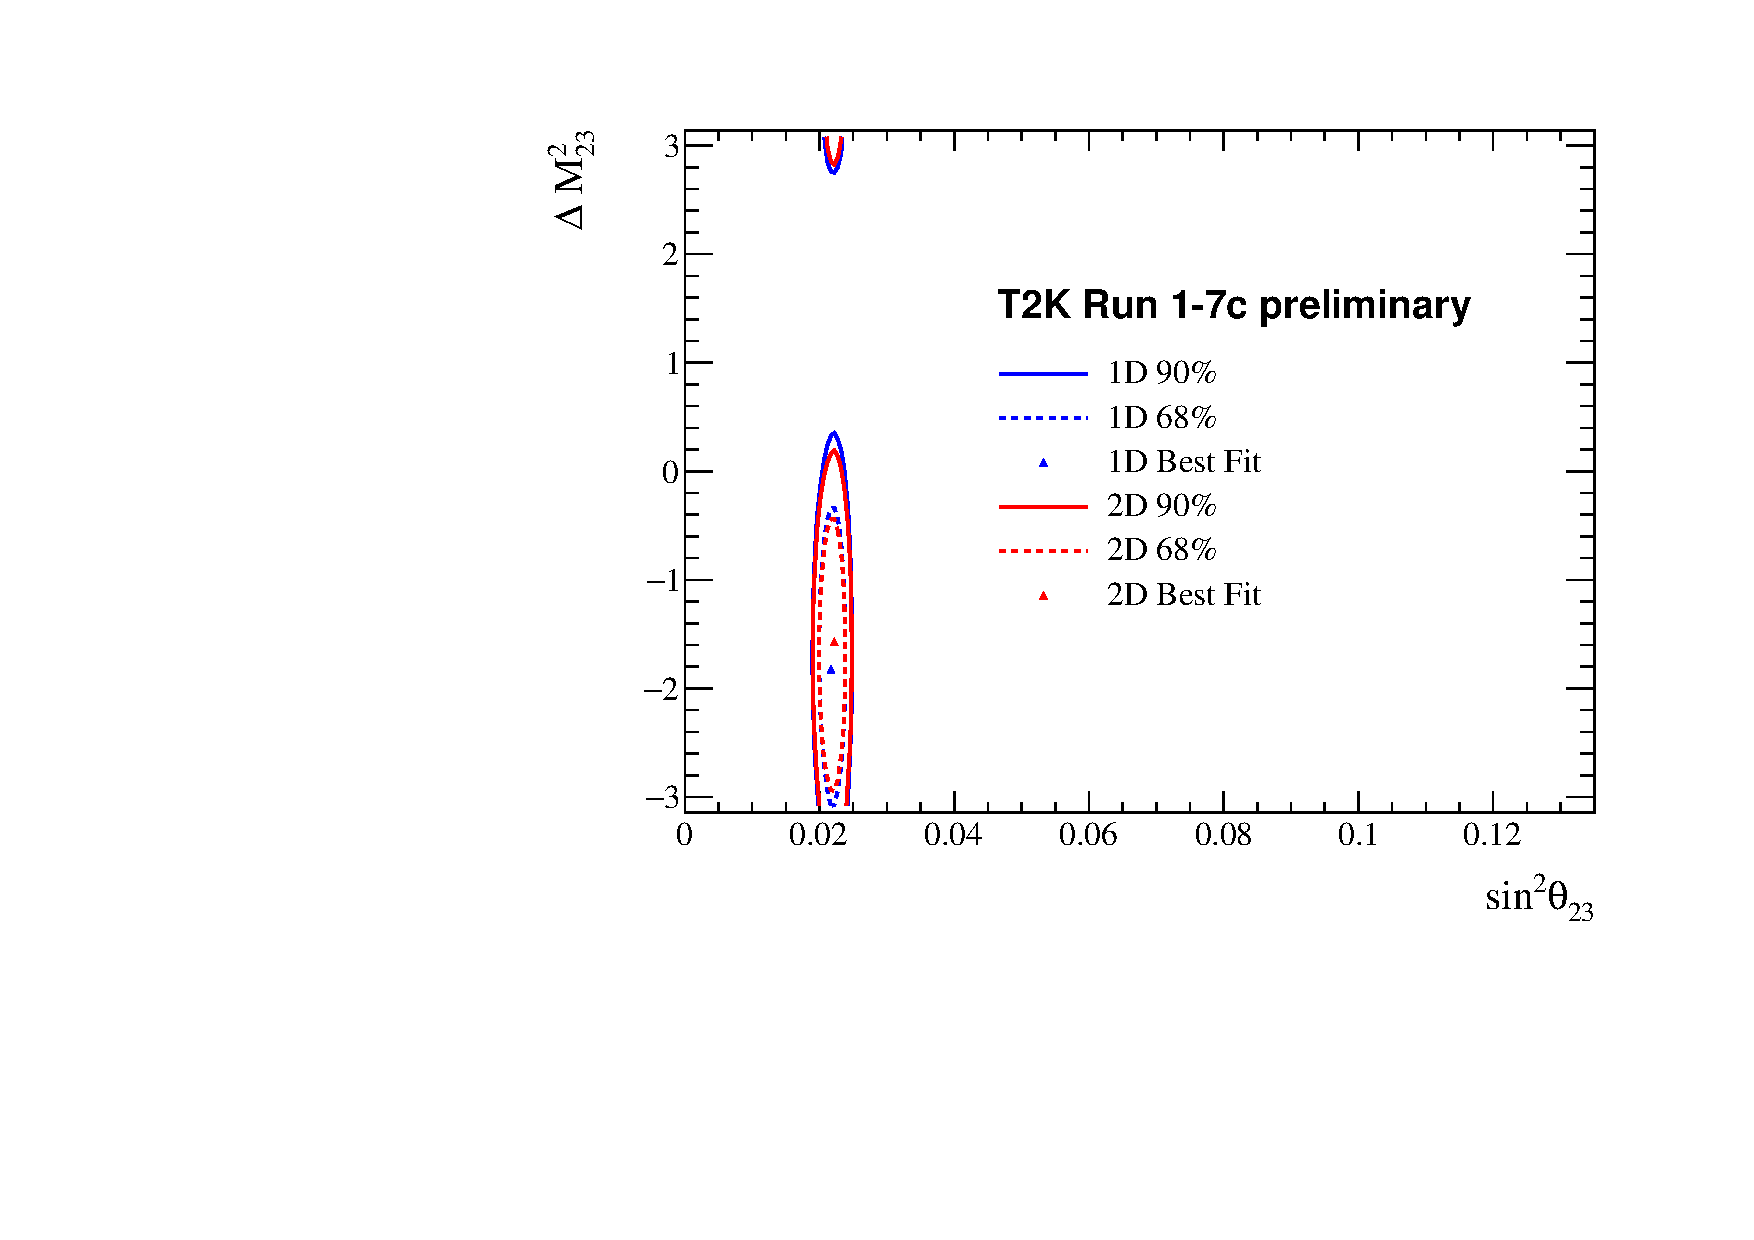
\includegraphics[width=\textwidth]{TalkPics/2Ddatafit_270916/contours_1D2Dcomparisons_wRC/comparedcontours_th13dcp_1Dvs2D_official.pdf}
    \end{columns}
  \end{frame}

  \begin{frame}
    \centering
    \begin{columns}
      \column{.6\textwidth}
      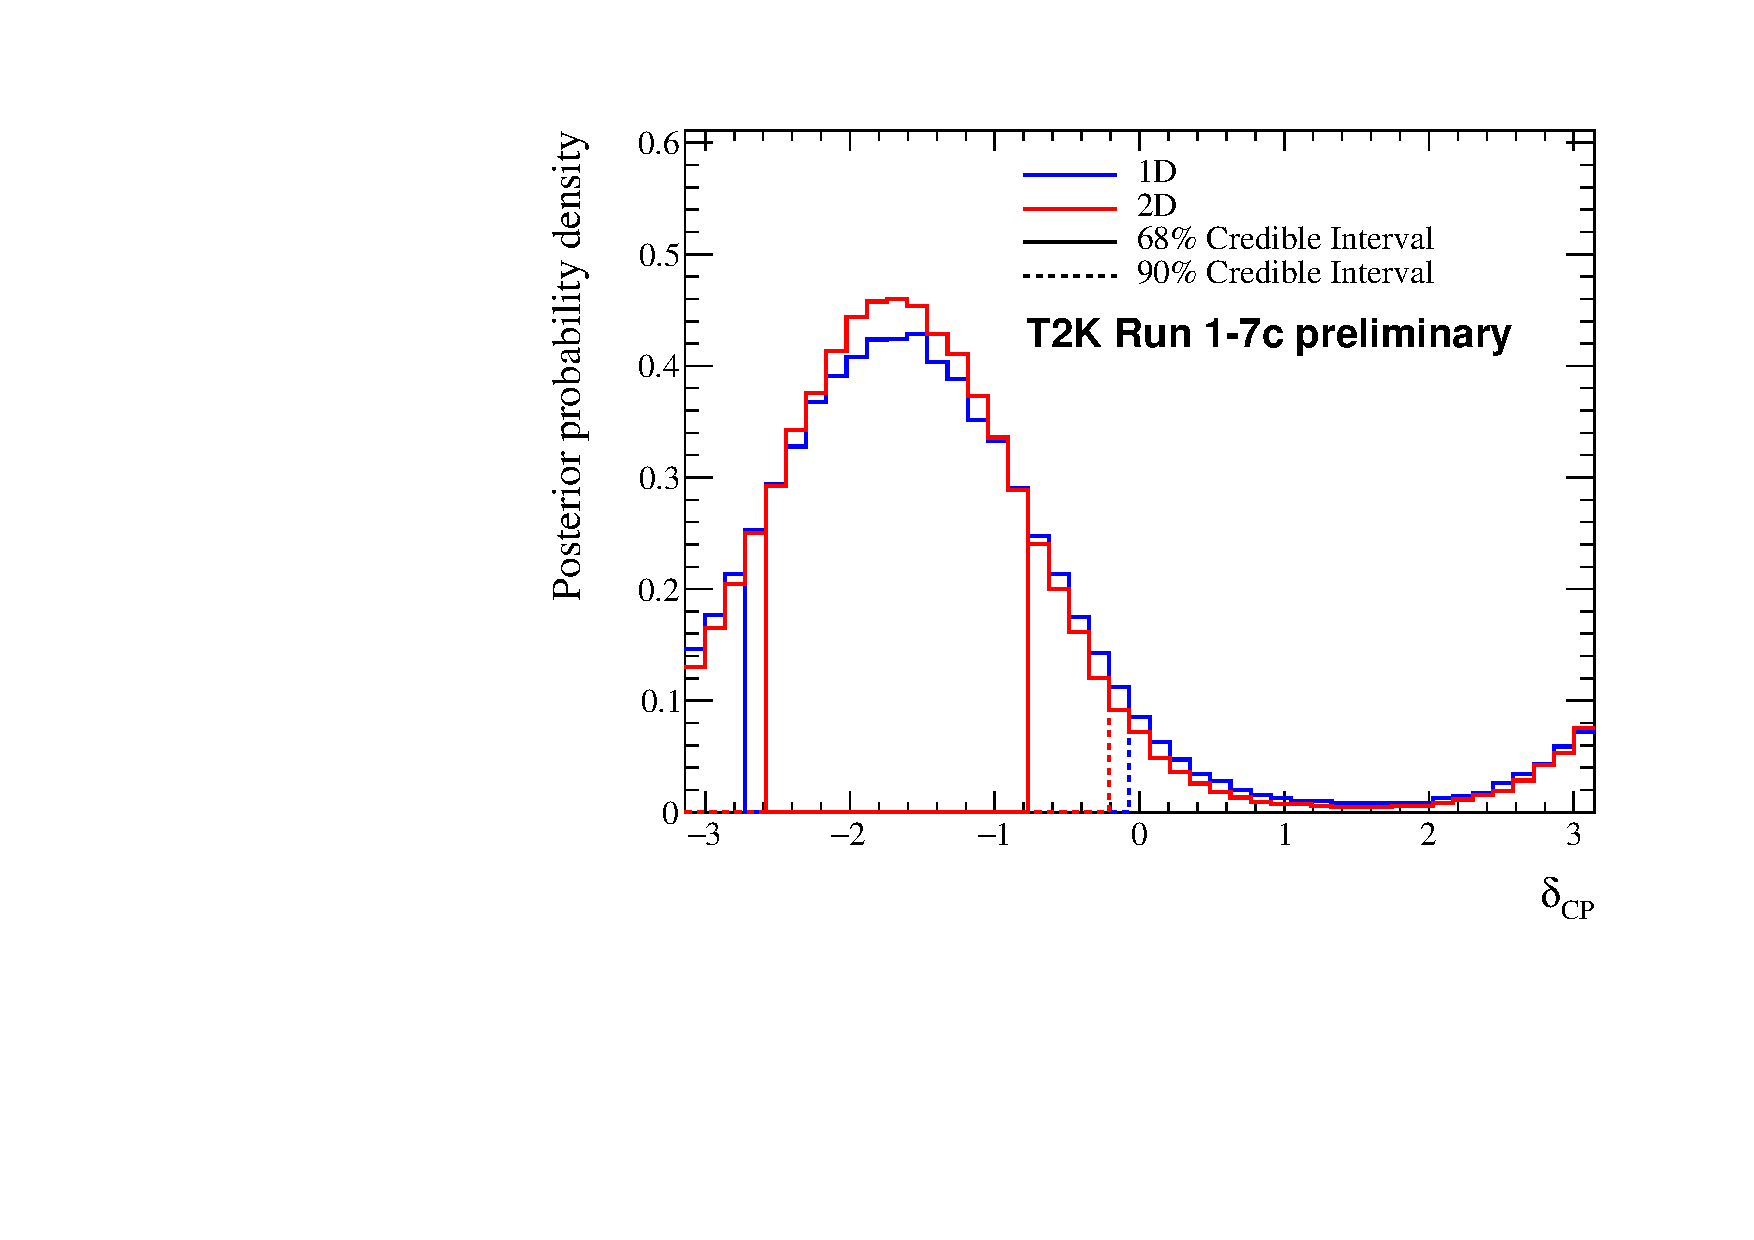
\includegraphics[width=\textwidth]{TalkPics/2Ddatafit_270916/contours_1D2Dcomparisons_wRC/contours_1D_dcp_compare_official.pdf}
    \end{columns}
  \end{frame}



  \begin{frame}
    \centering
    \huge\textcolor{beamer@icmiddleblue}{MaCh3-Valor comparisons woRC}
  \end{frame}

  \begin{frame}
    \centering
    \frametitle{Disappearance parameters}
    \begin{columns}
      \column{.6\textwidth}
      \textcolor{beamer@icmiddleblue}{NH}

    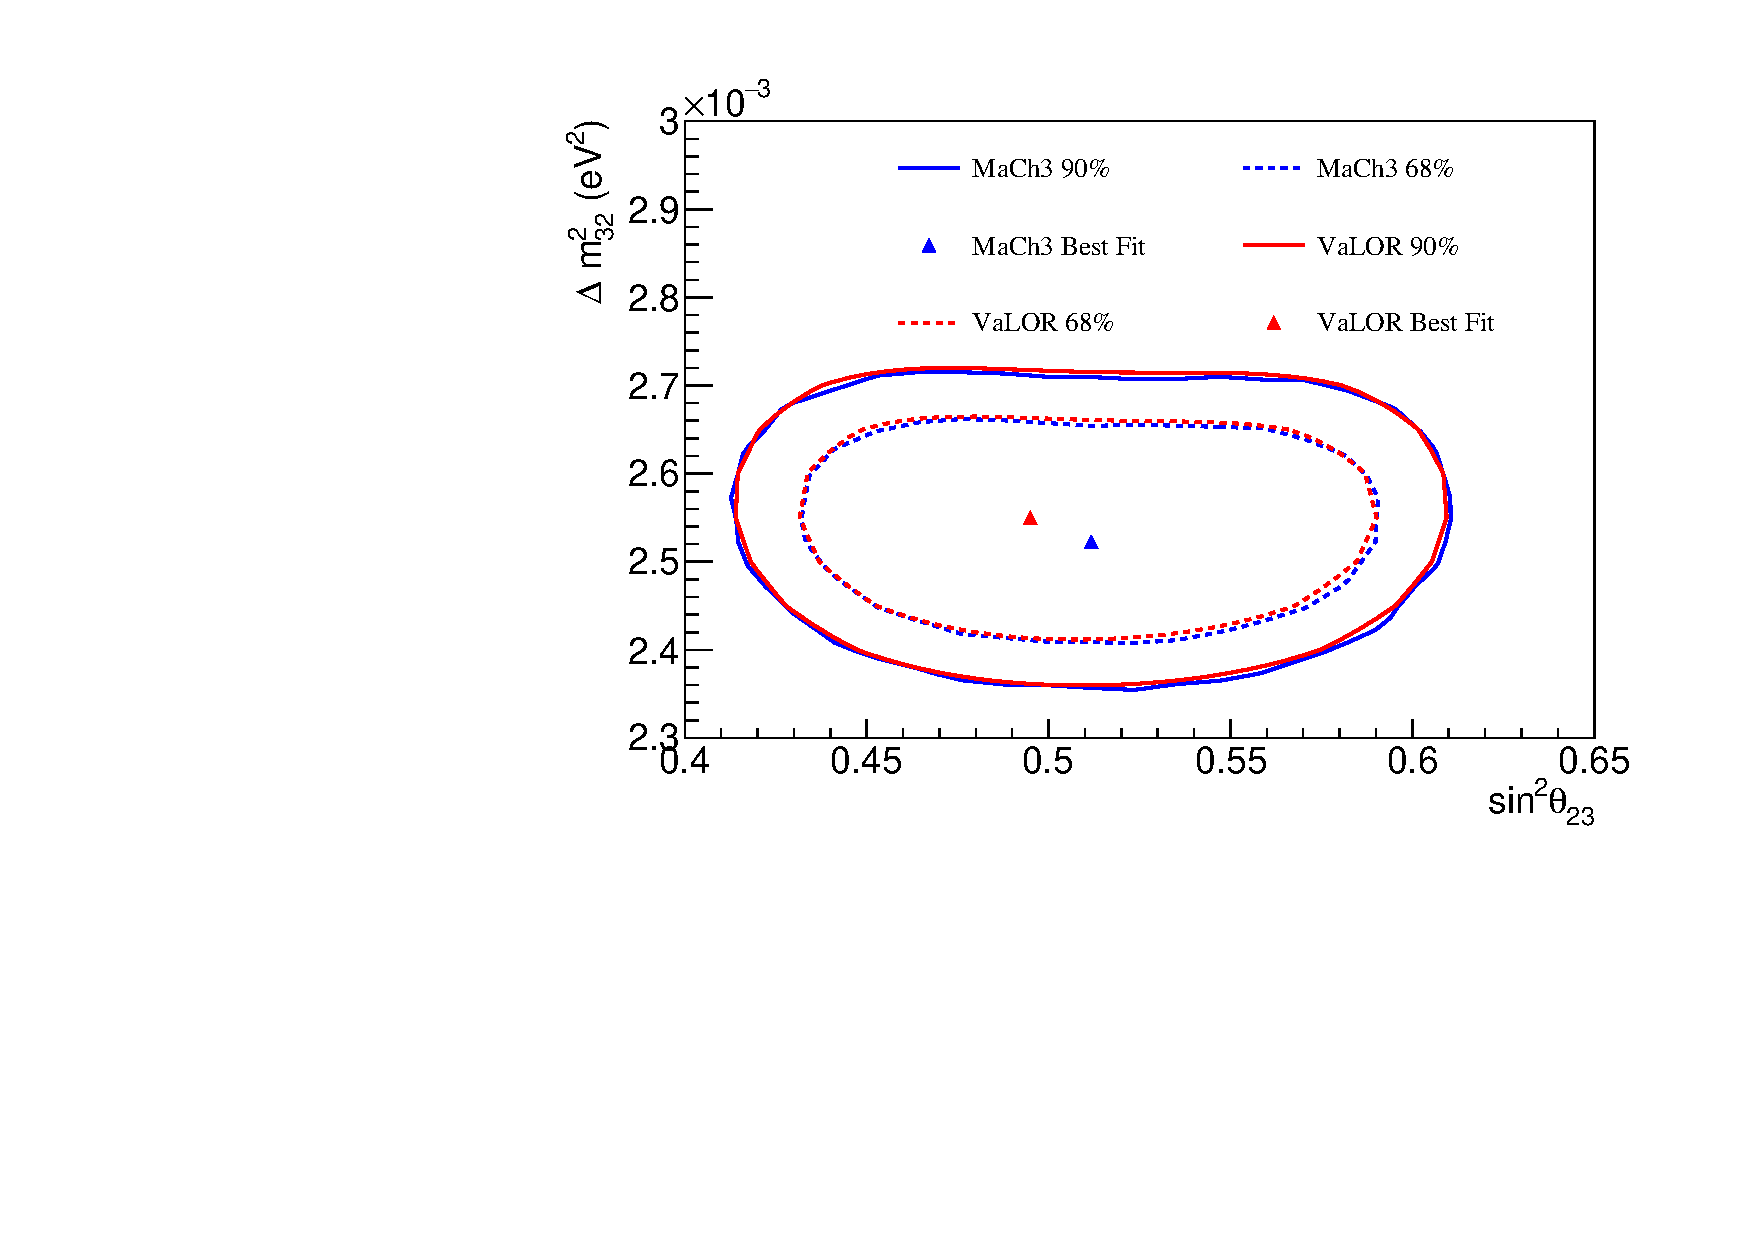
\includegraphics[width=\textwidth]{TalkPics/2Ddatafit_270916/comparedcontours_2D_mach3valor_woRC_NH.pdf}
      \column{.6\textwidth}
      \textcolor{beamer@icmiddleblue}{IH}

      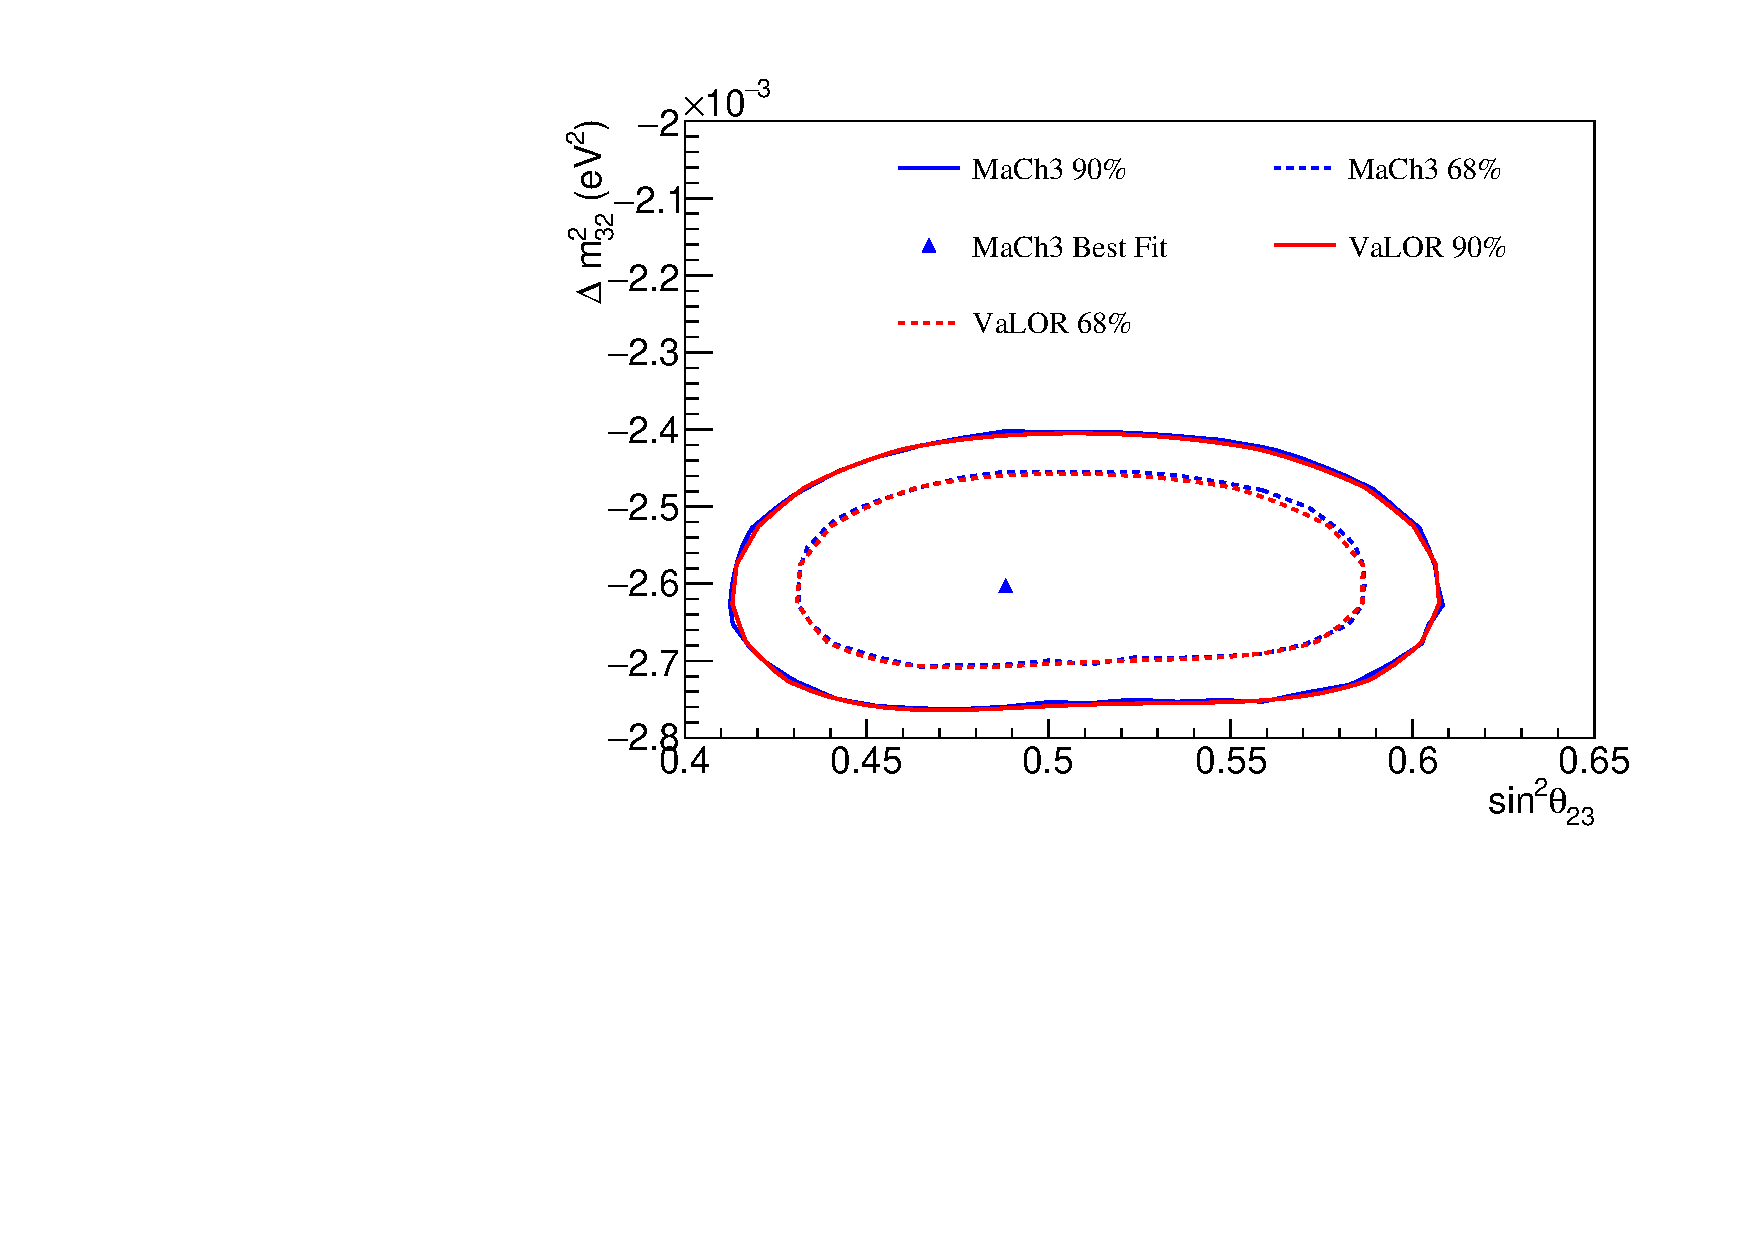
\includegraphics[width=\textwidth]{TalkPics/2Ddatafit_270916/comparedcontours_2D_mach3valor_woRC_IH.pdf}
    \end{columns}
  \end{frame}

  \begin{frame}
    \centering
    \frametitle{Appearance parameters}
    \begin{columns}
      \column{.6\textwidth}
      \textcolor{beamer@icmiddleblue}{NH}

    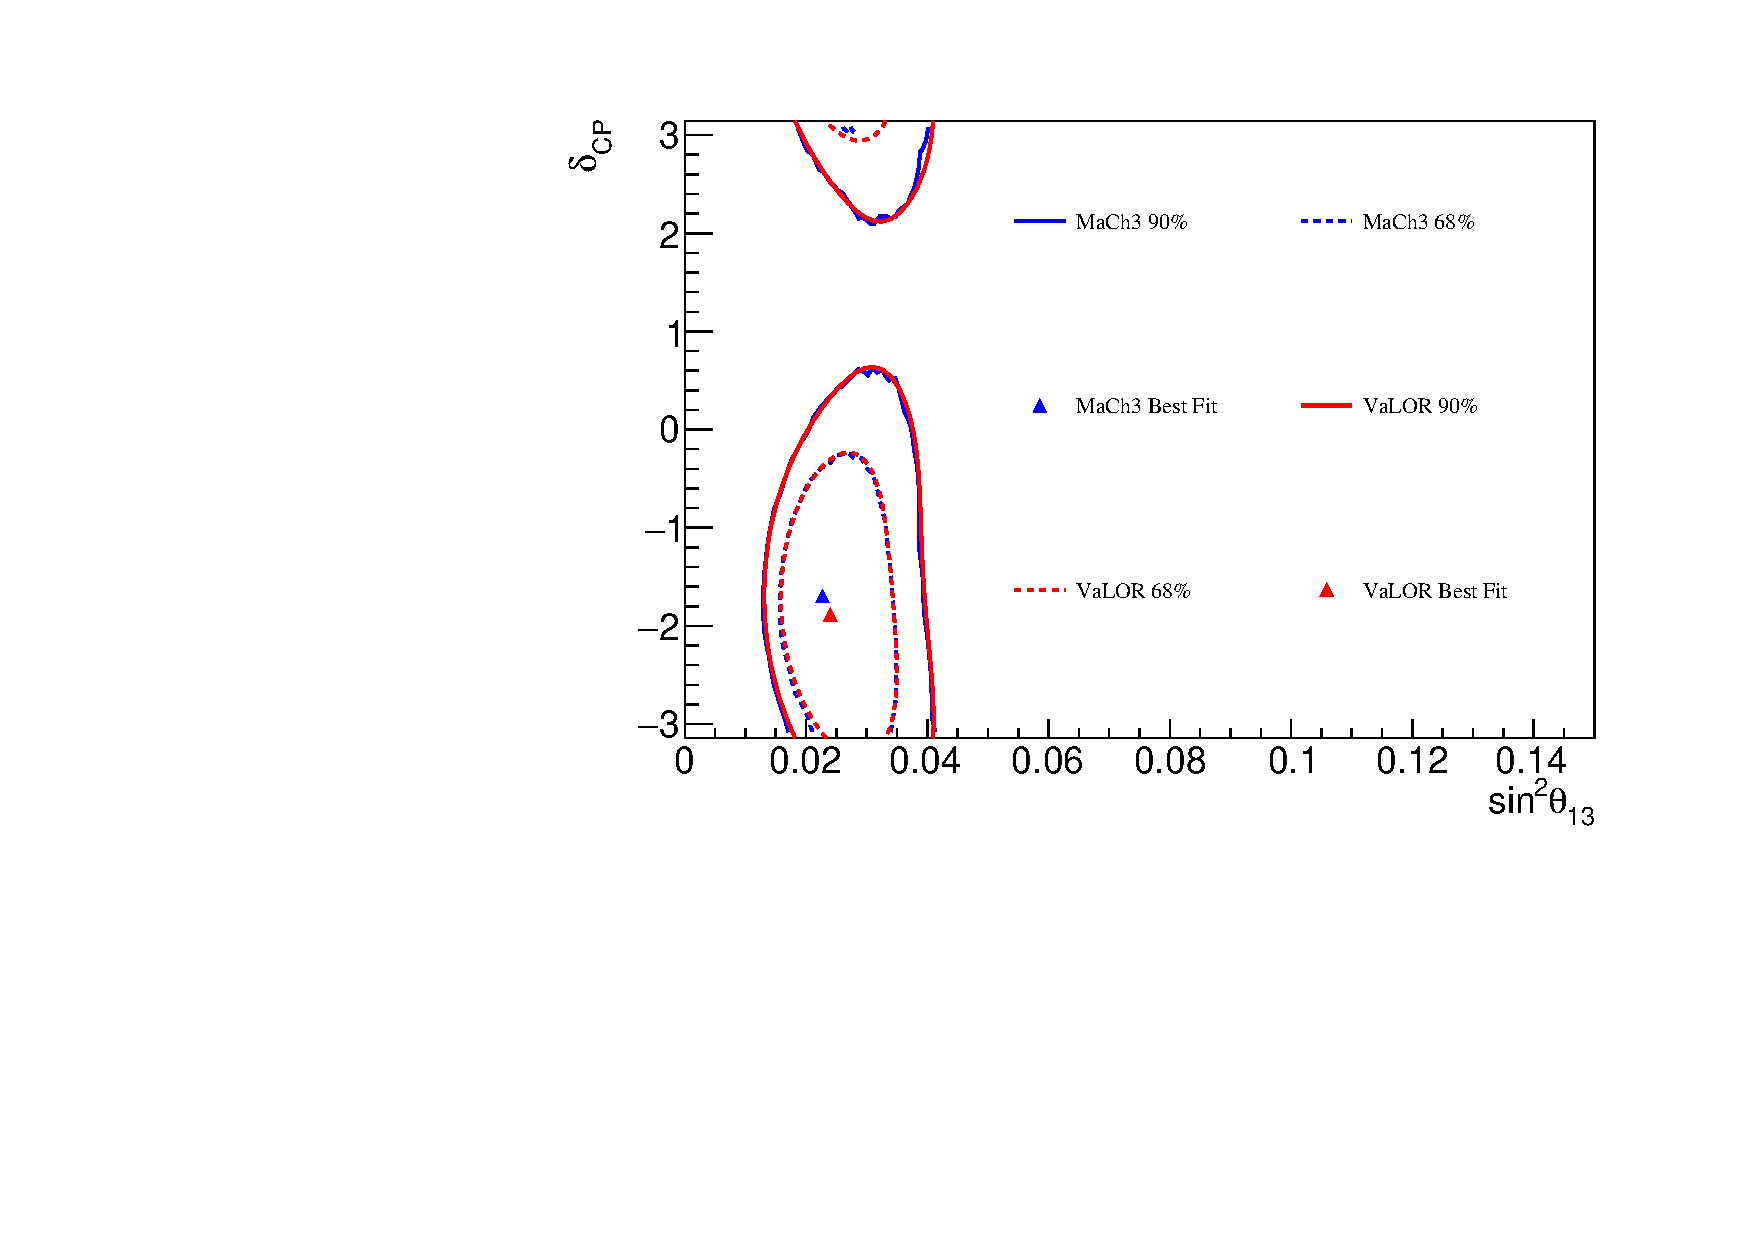
\includegraphics[width=\textwidth]{TalkPics/2Ddatafit_270916/comparedcontours_2D_mach3valor_woRC_th13dcp_NH.pdf}
      \column{.6\textwidth}
      \textcolor{beamer@icmiddleblue}{IH}

      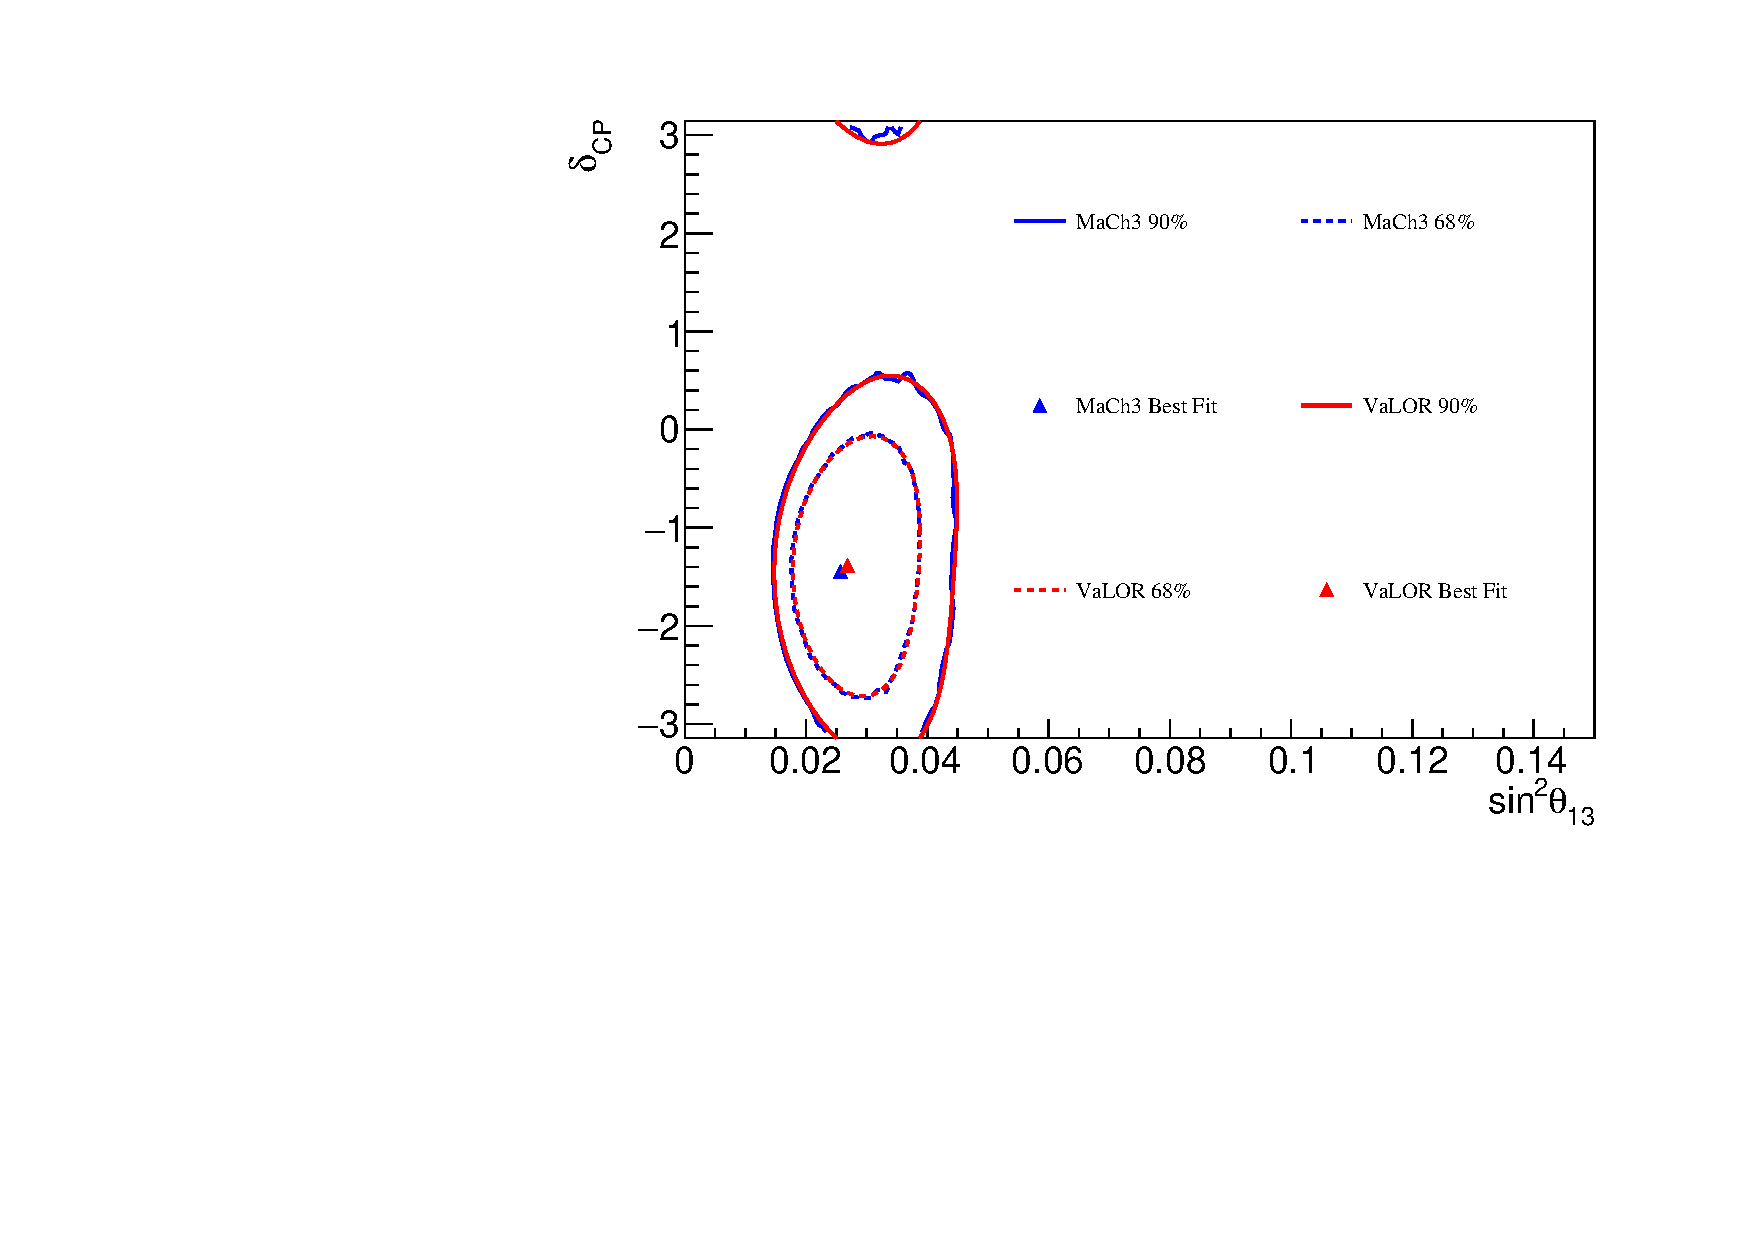
\includegraphics[width=\textwidth]{TalkPics/2Ddatafit_270916/comparedcontours_2D_mach3valor_woRC_th13dcp_IH.pdf}
    \end{columns}
  \end{frame}

  \begin{frame}
    \centering
    \frametitle{$\delta_{CP}$}
    \begin{columns}
      \column{.6\textwidth}
      \textcolor{beamer@icmiddleblue}{NH}

    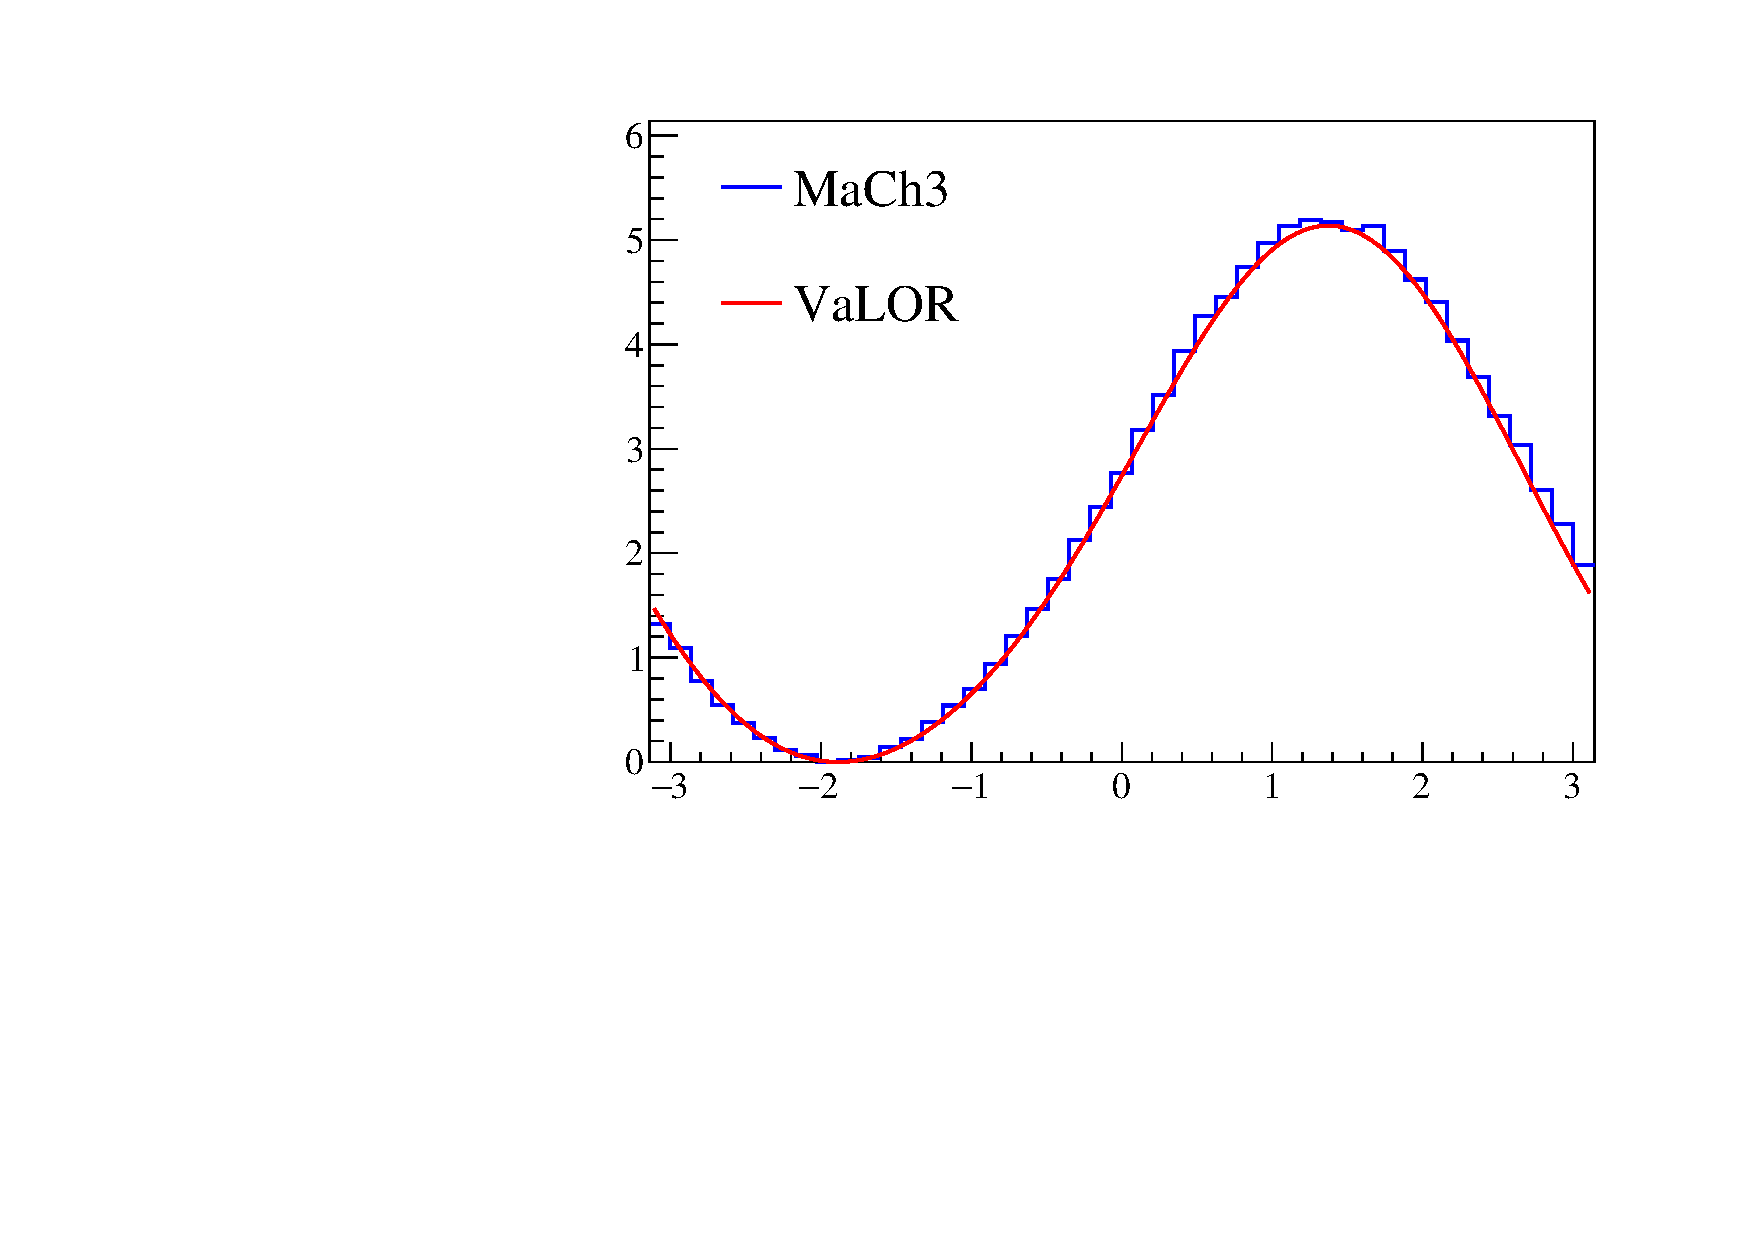
\includegraphics[width=\textwidth]{TalkPics/2Ddatafit_270916/comparedcontours_2D_mach3valor_woRC_dcp_NH.pdf}
      \column{.6\textwidth}
      \textcolor{beamer@icmiddleblue}{IH}

      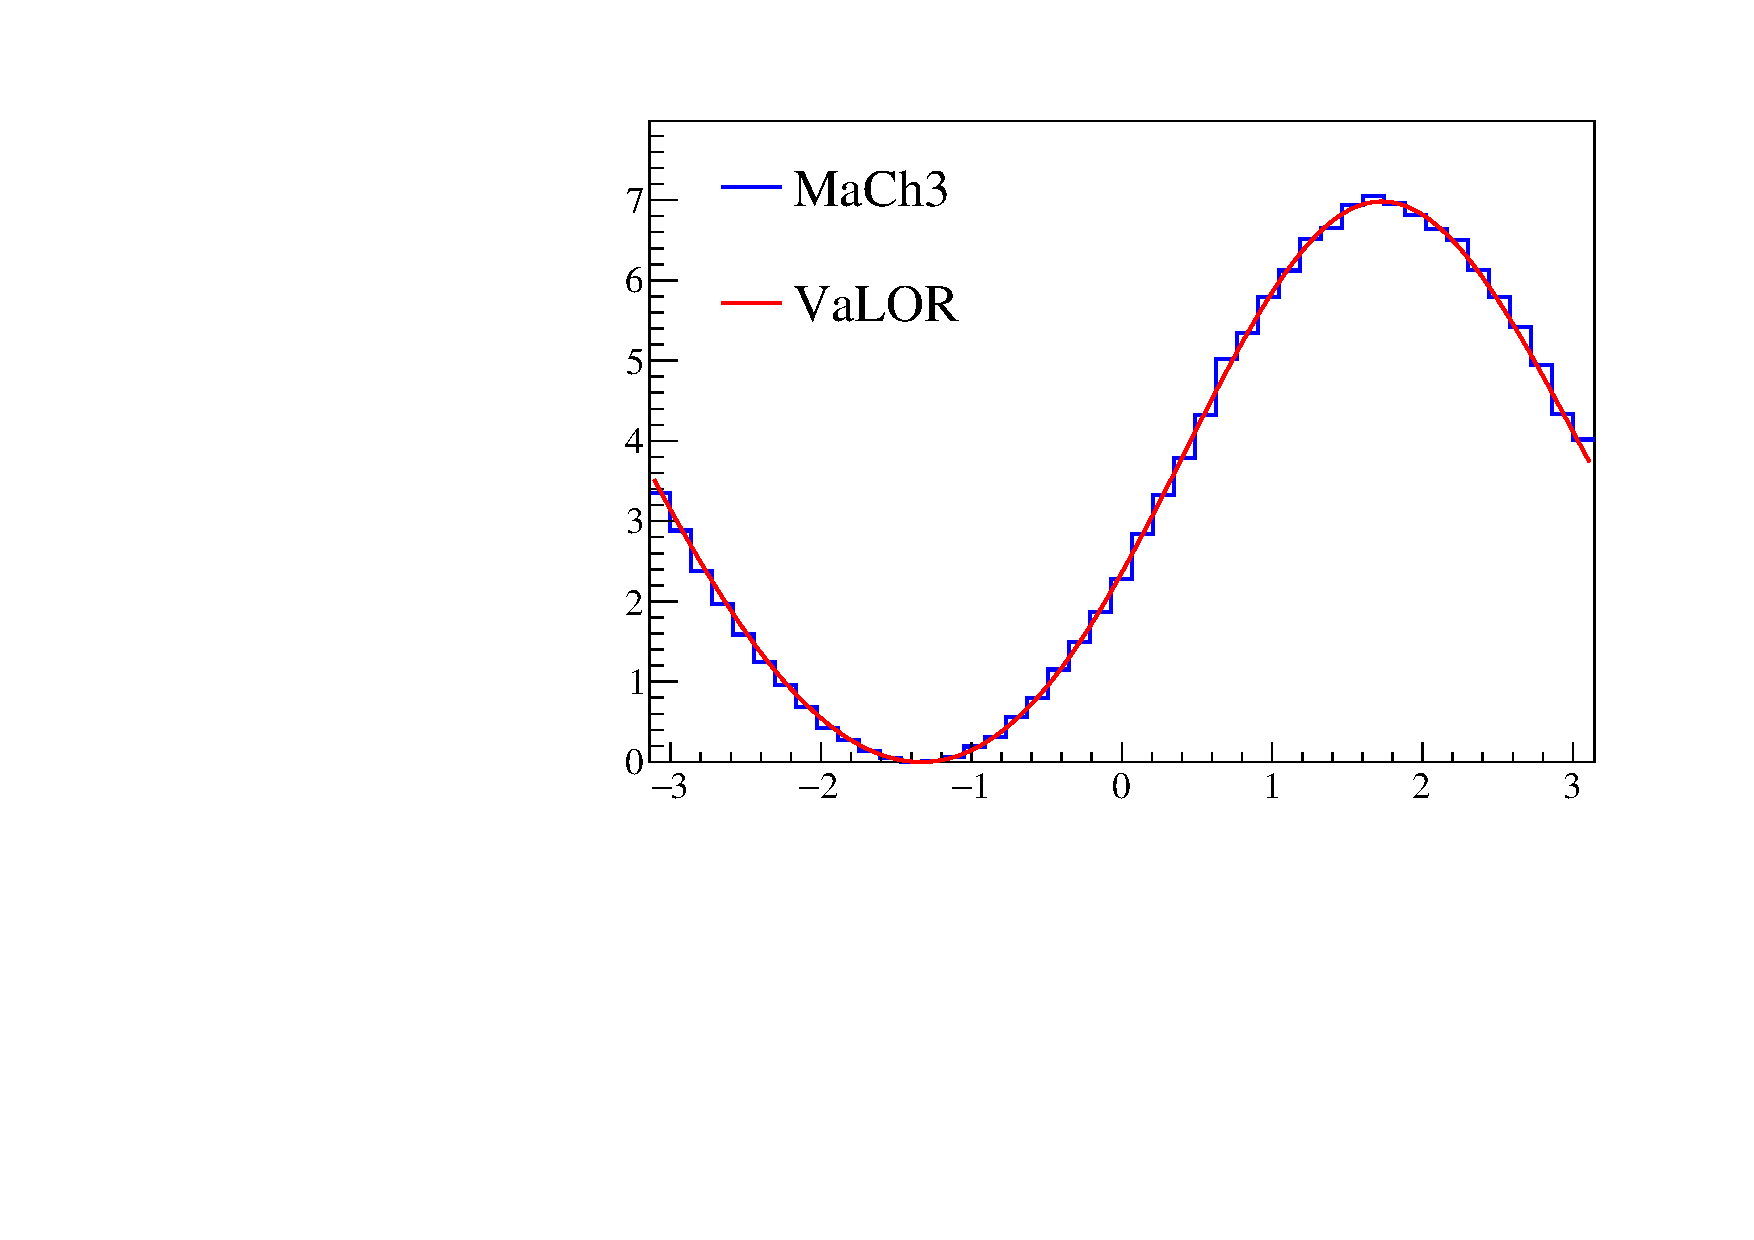
\includegraphics[width=\textwidth]{TalkPics/2Ddatafit_270916/comparedcontours_2D_mach3valor_woRC_dcp_IH.pdf}
    \end{columns}
  \end{frame}

  \begin{frame}
    \centering
    \huge\textcolor{beamer@icmiddleblue}{MaCh3-Valor comparisons wRC}
  \end{frame}
  \begin{frame}
    \centering
    \frametitle{Disappearance parameters}
    \begin{columns}
      \column{.6\textwidth}
      \textcolor{beamer@icmiddleblue}{NH}

    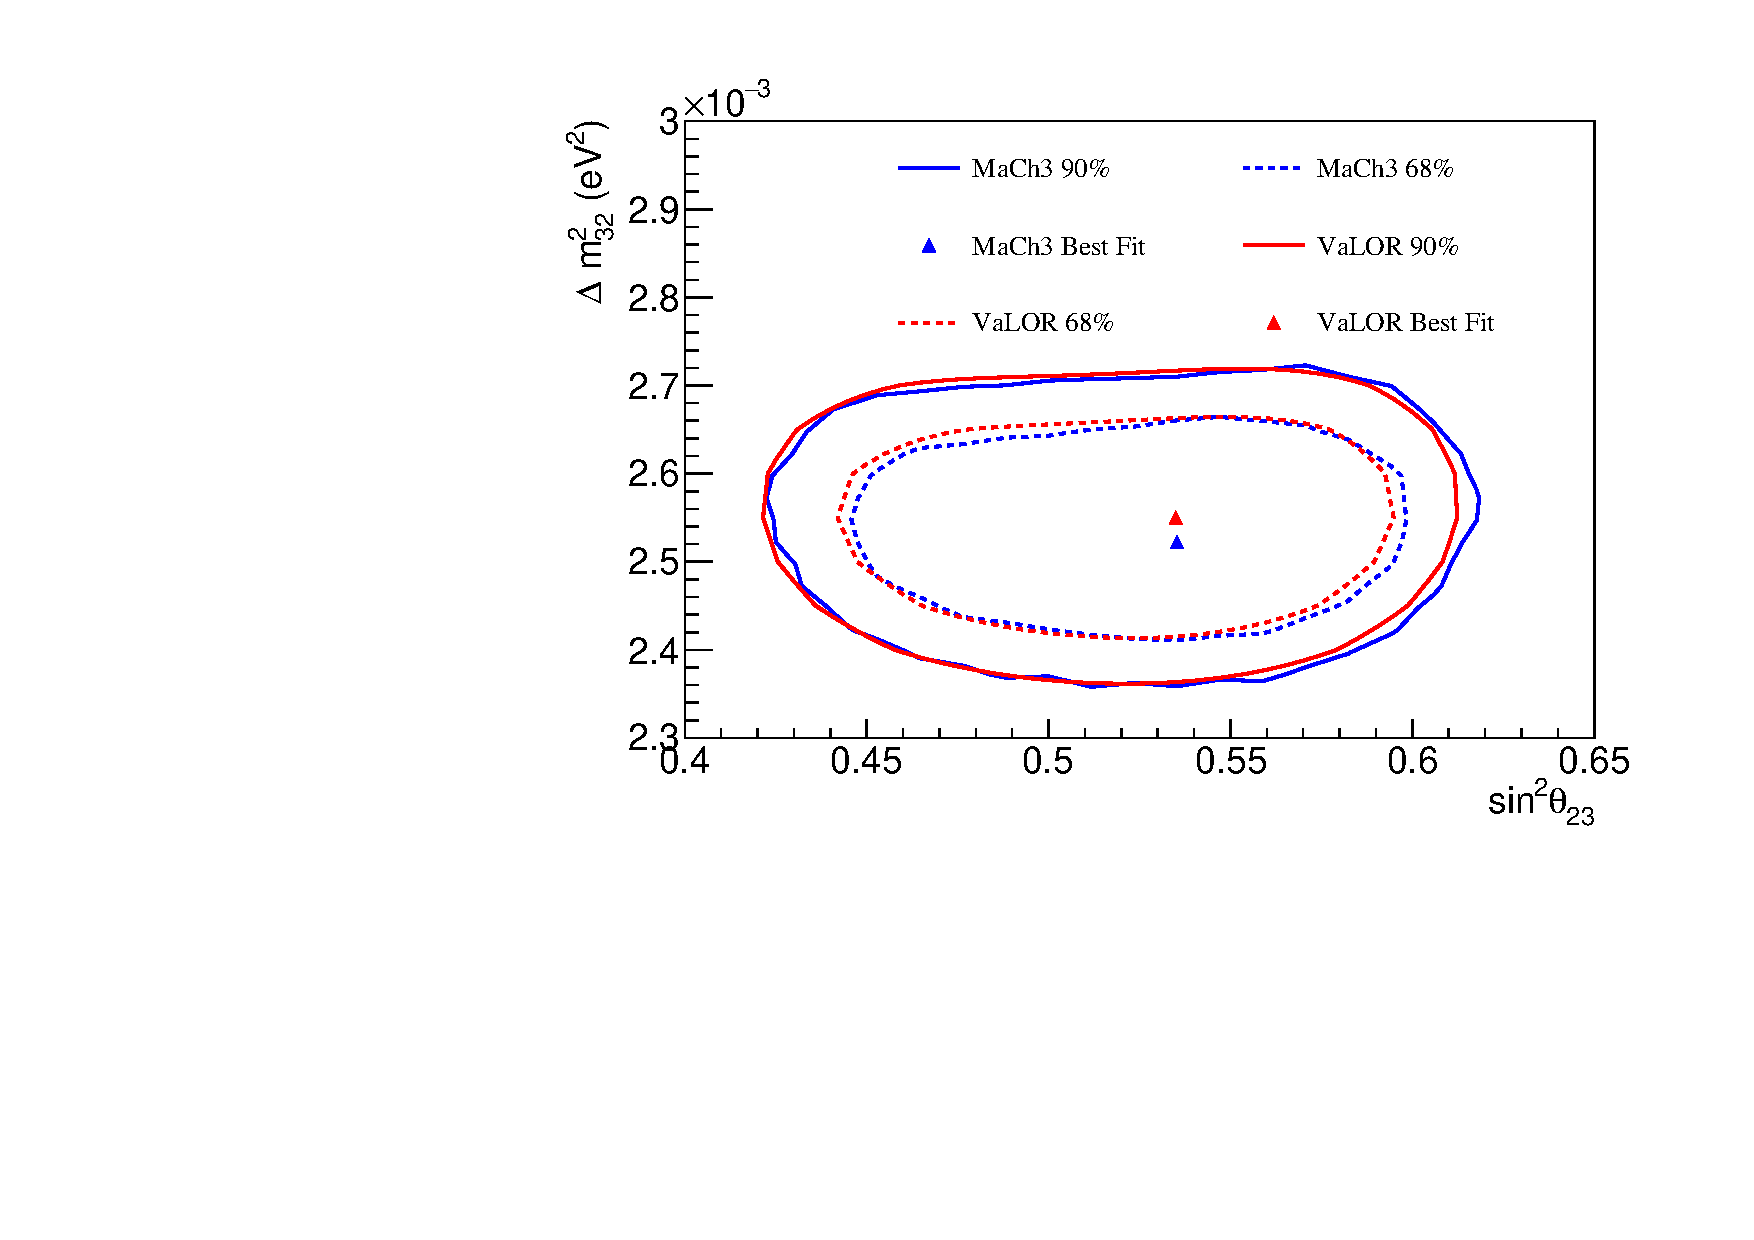
\includegraphics[width=\textwidth]{TalkPics/2Ddatafit_270916/comparedcontours_2D_mach3valor_wRC_NH.pdf}
      \column{.6\textwidth}
      \textcolor{beamer@icmiddleblue}{IH}

      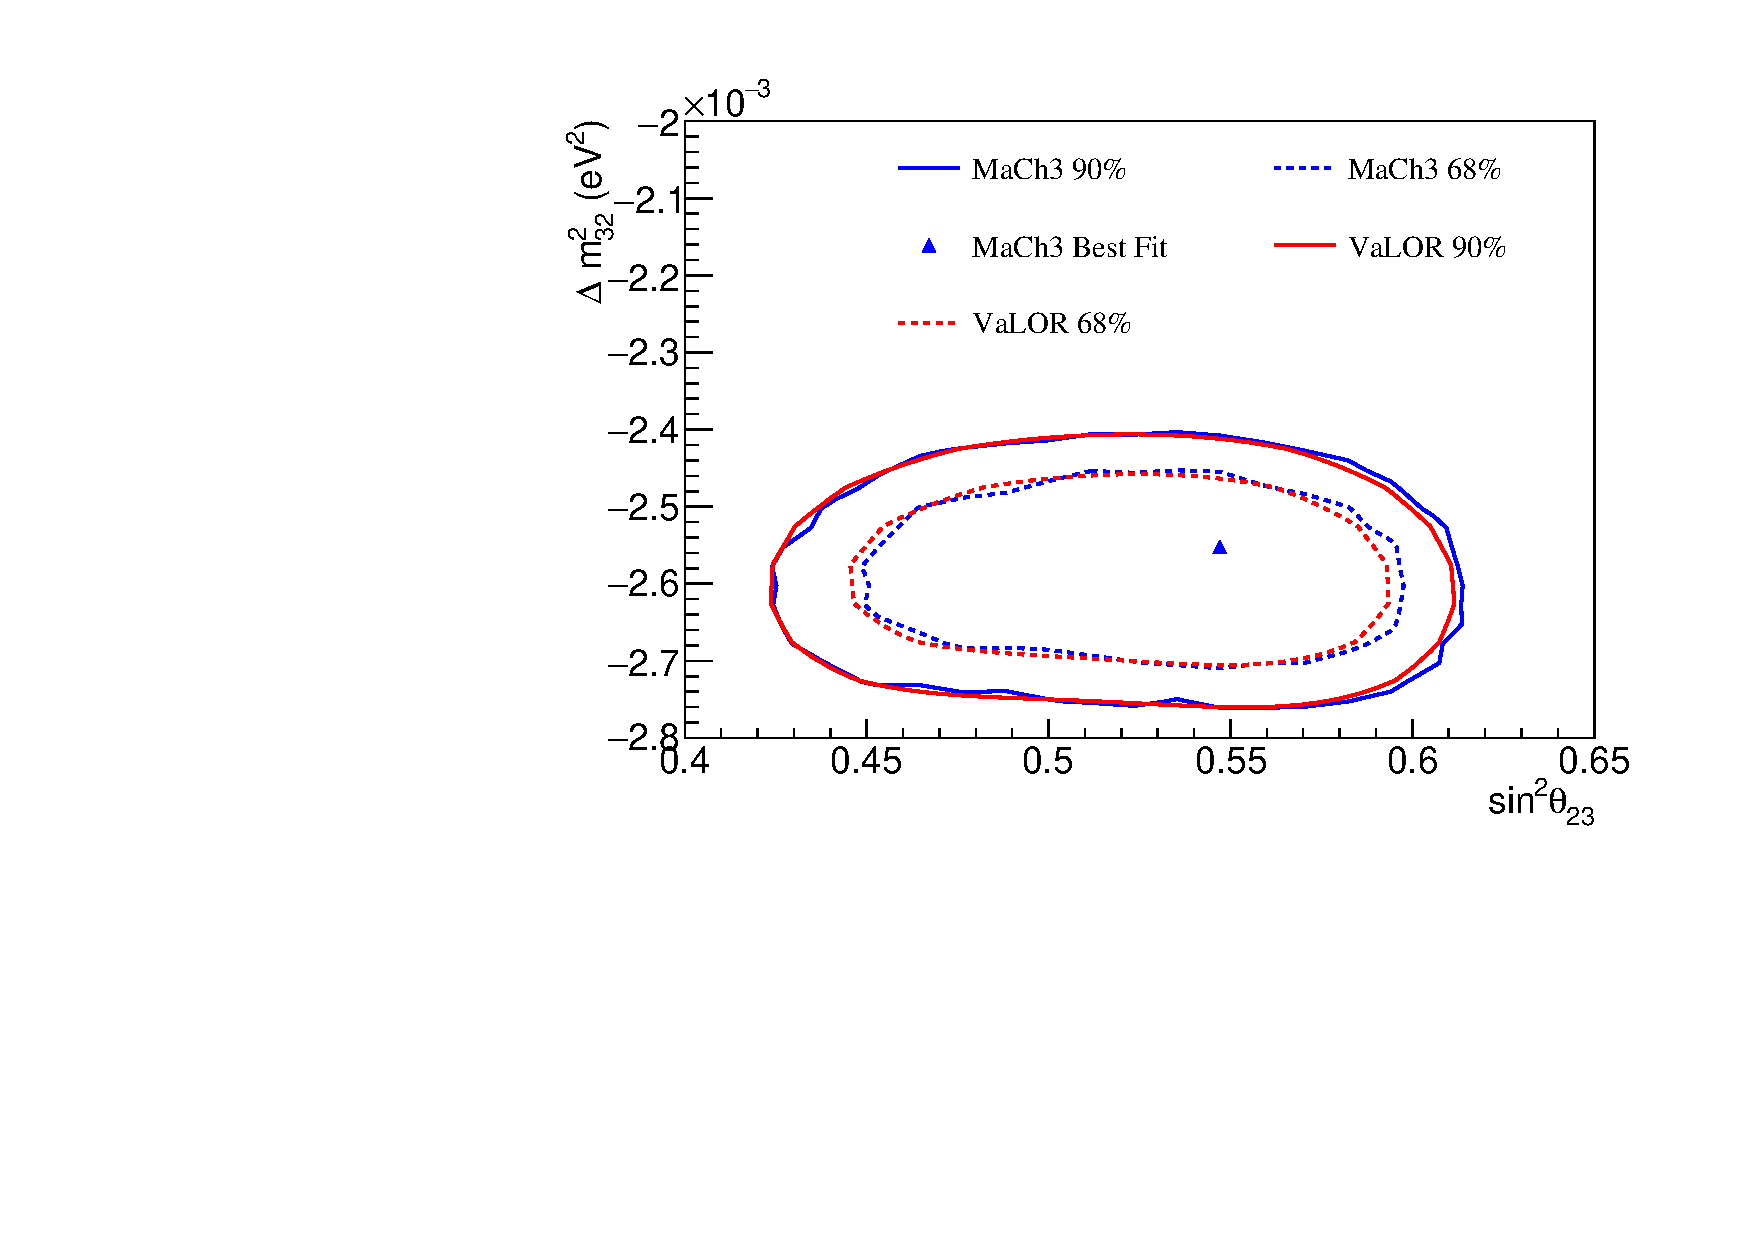
\includegraphics[width=\textwidth]{TalkPics/2Ddatafit_270916/comparedcontours_2D_mach3valor_wRC_IH.pdf}
    \end{columns}
  \end{frame}

  \begin{frame}
    \centering
    \frametitle{Appearance parameters}
    \begin{columns}
      \column{.6\textwidth}
      \textcolor{beamer@icmiddleblue}{NH}

    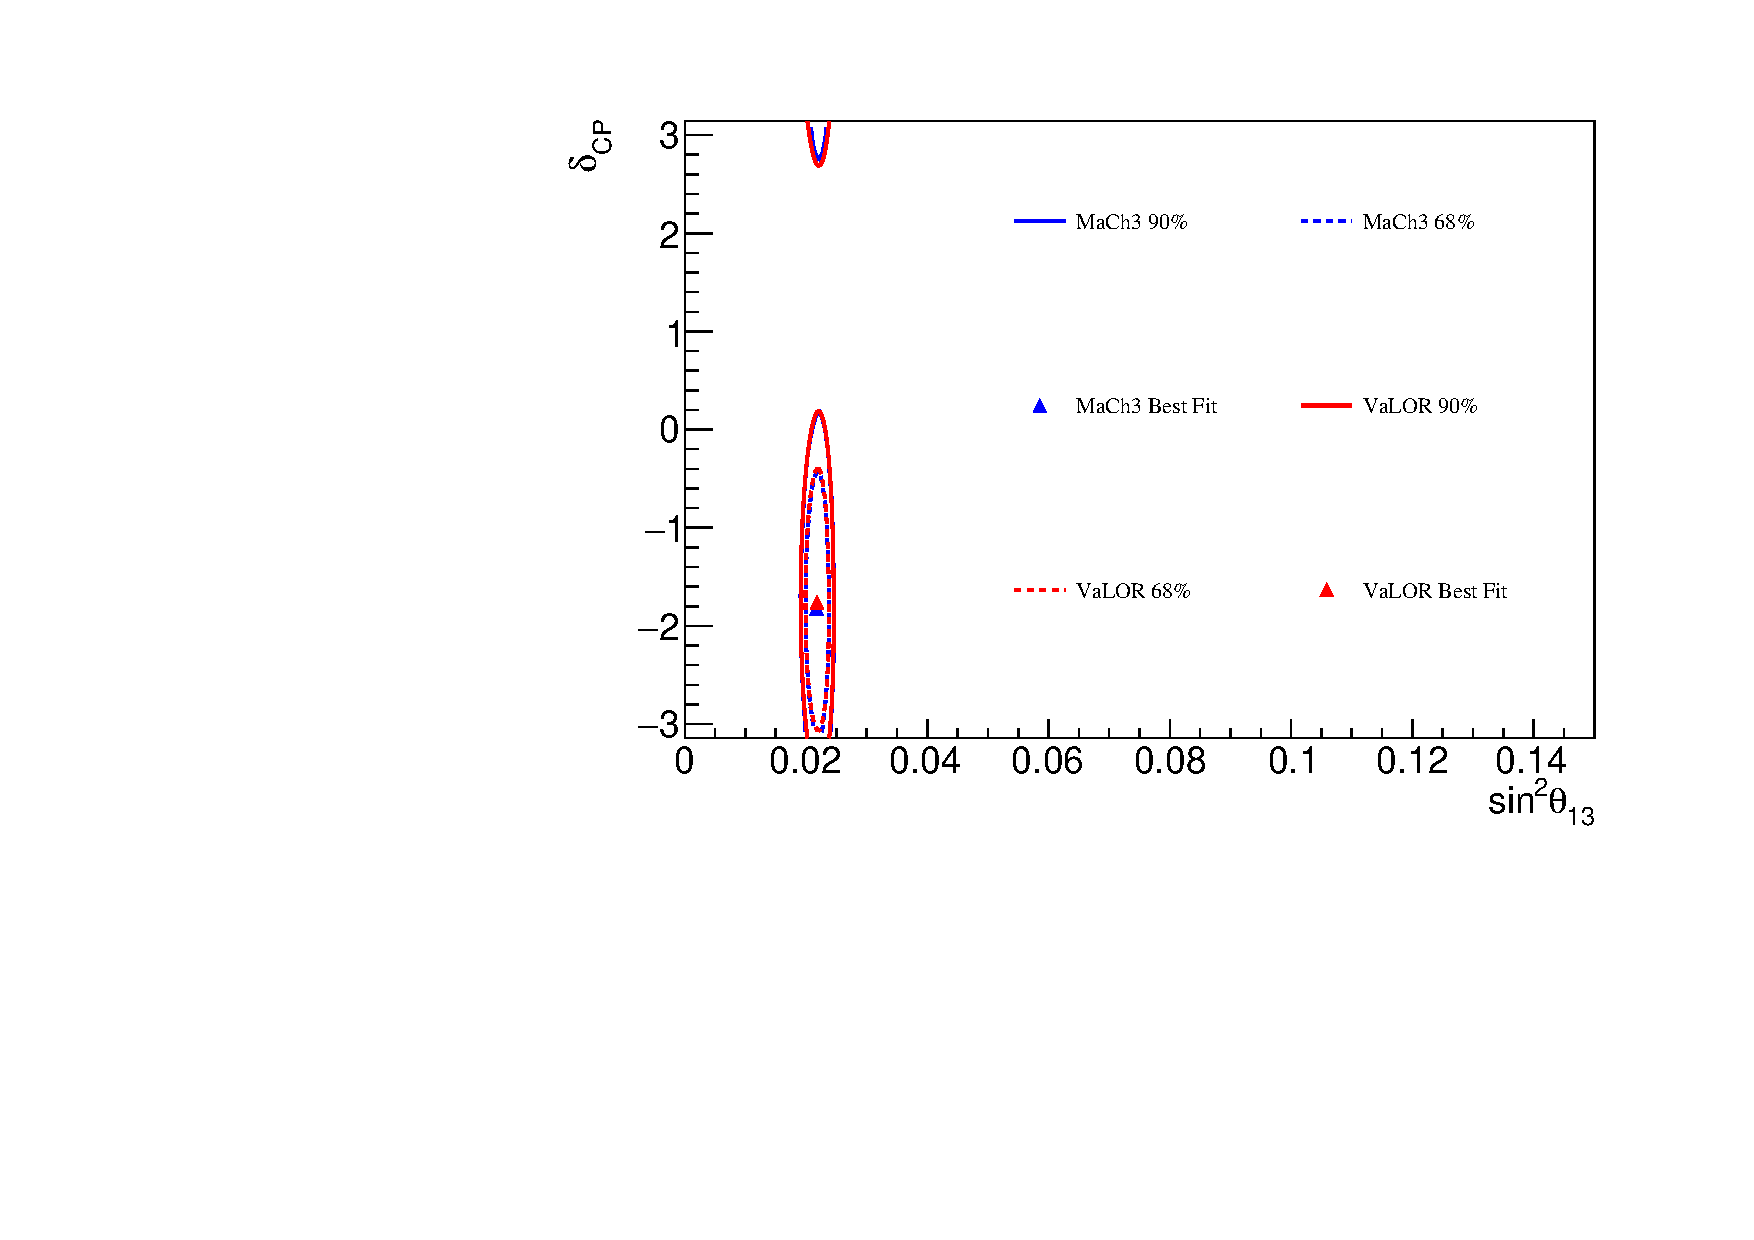
\includegraphics[width=\textwidth]{TalkPics/2Ddatafit_270916/comparedcontours_2D_mach3valor_wRC_th13dcp_NH.pdf}
      \column{.6\textwidth}
      \textcolor{beamer@icmiddleblue}{IH}

      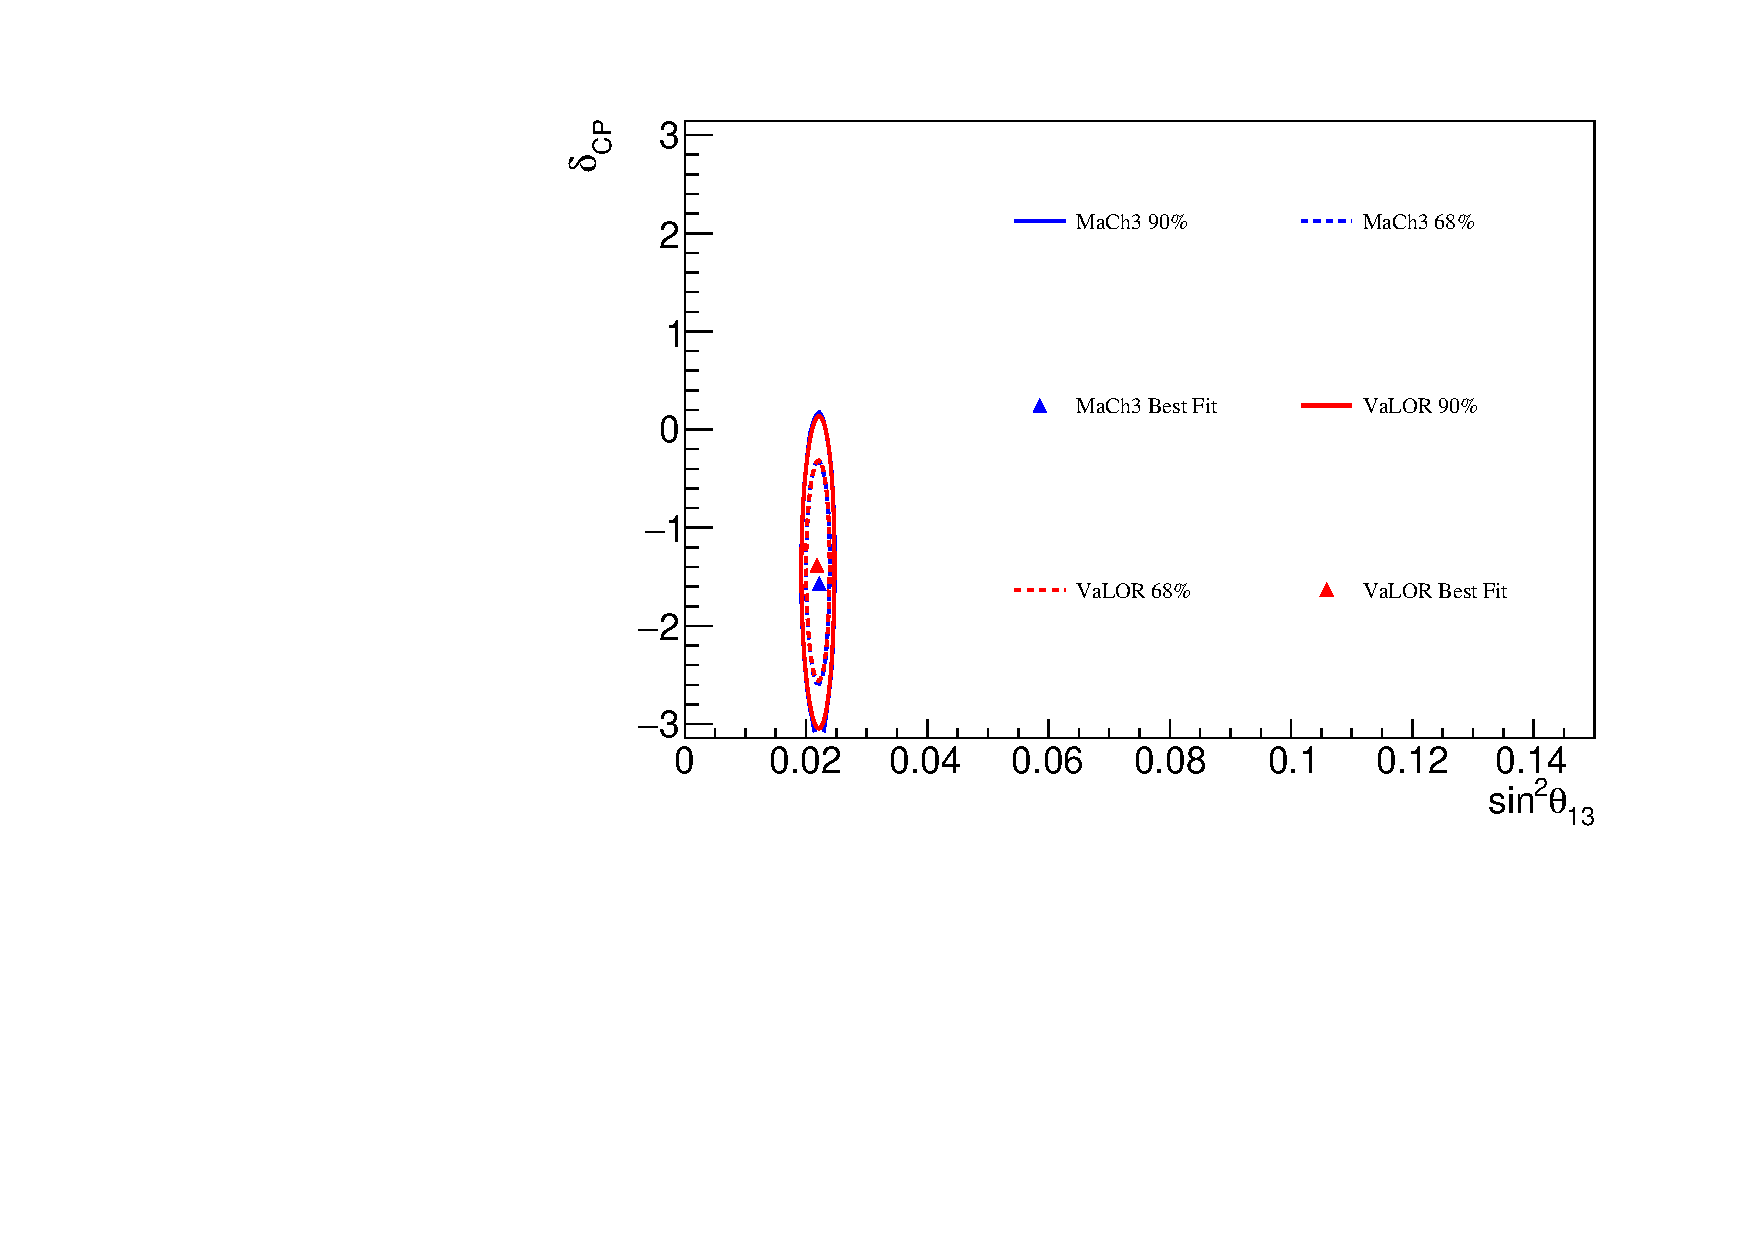
\includegraphics[width=\textwidth]{TalkPics/2Ddatafit_270916/comparedcontours_2D_mach3valor_wRC_th13dcp_IH.pdf}
    \end{columns}
  \end{frame}

  \begin{frame}
    \centering
    \frametitle{$\delta_{CP}$}
    \begin{columns}
      \column{.6\textwidth}
      \textcolor{beamer@icmiddleblue}{NH}

    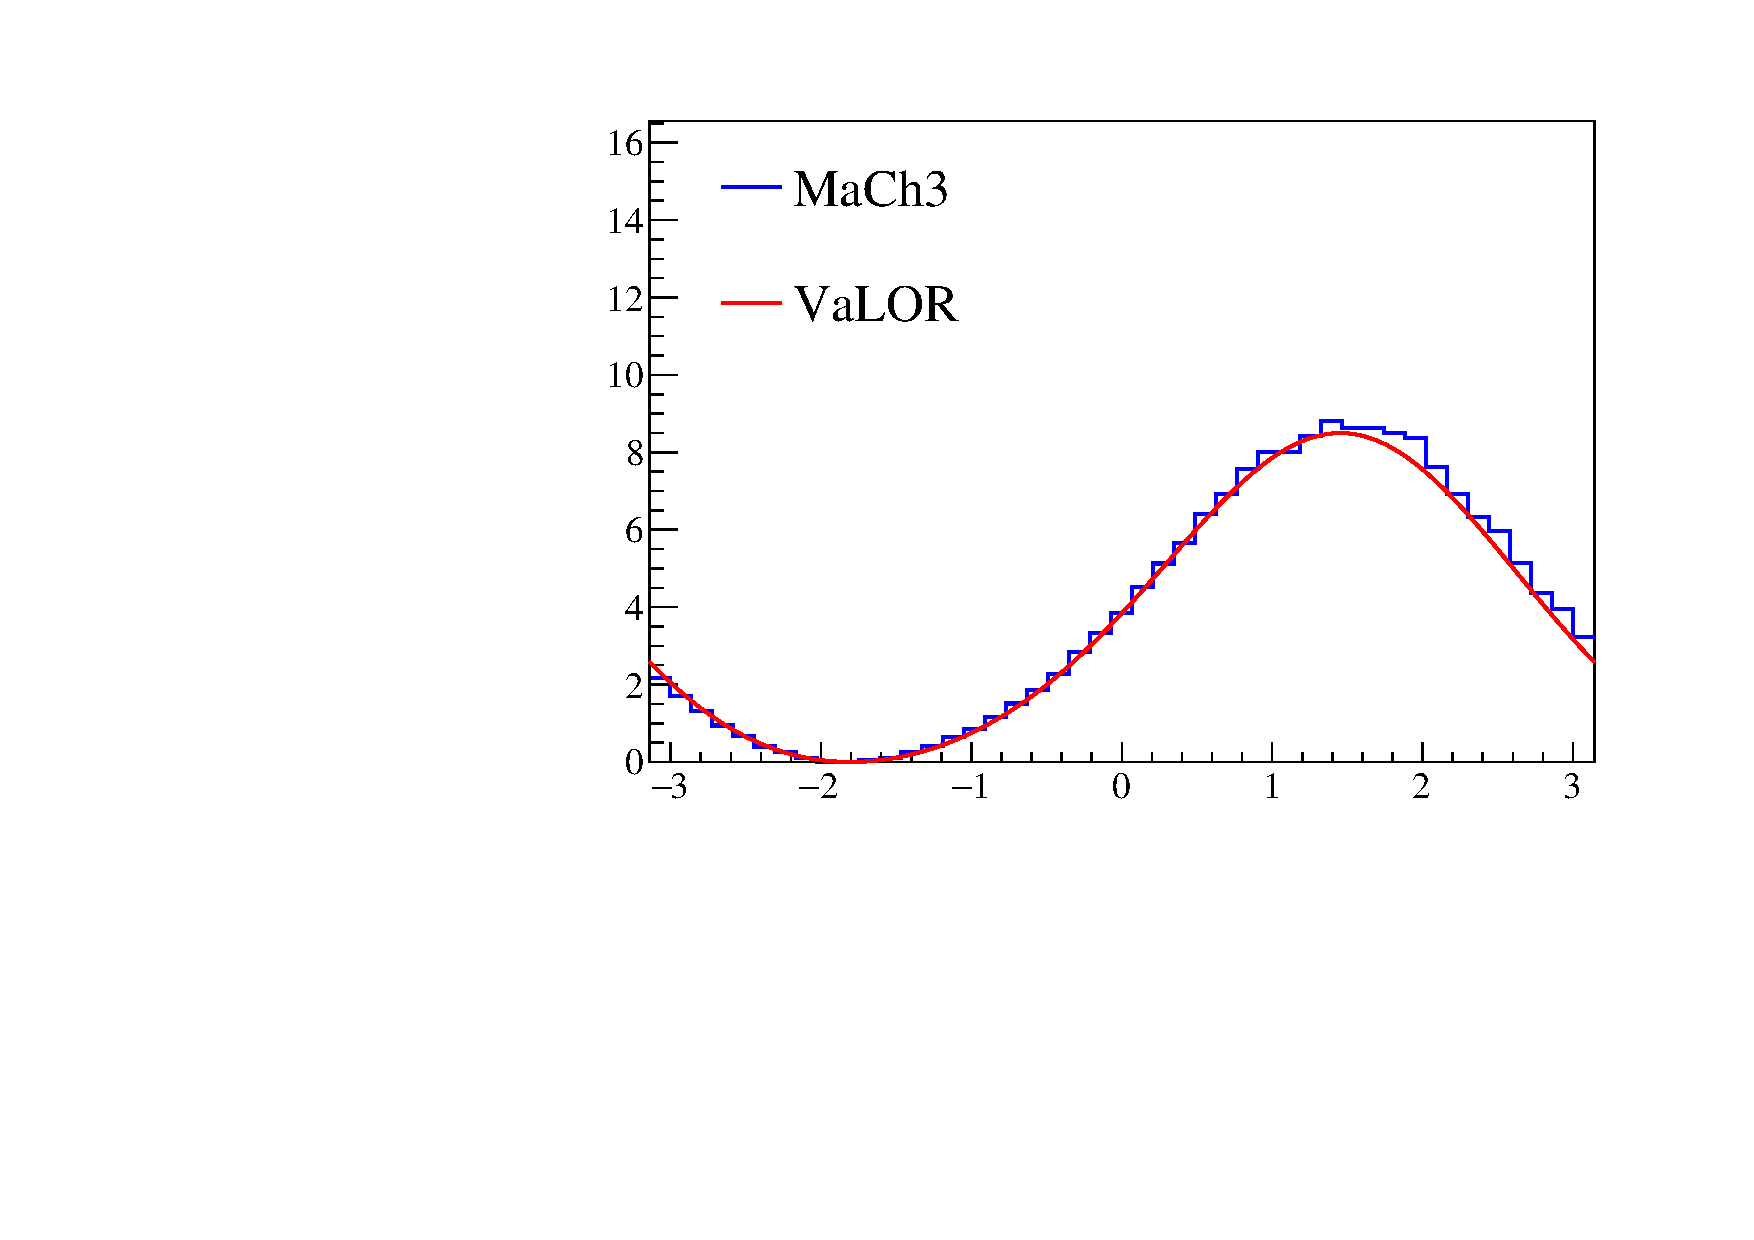
\includegraphics[width=\textwidth]{TalkPics/2Ddatafit_270916/comparedcontours_2D_mach3valor_wRC_dcp_NH.pdf}
      \column{.6\textwidth}
      \textcolor{beamer@icmiddleblue}{IH}

      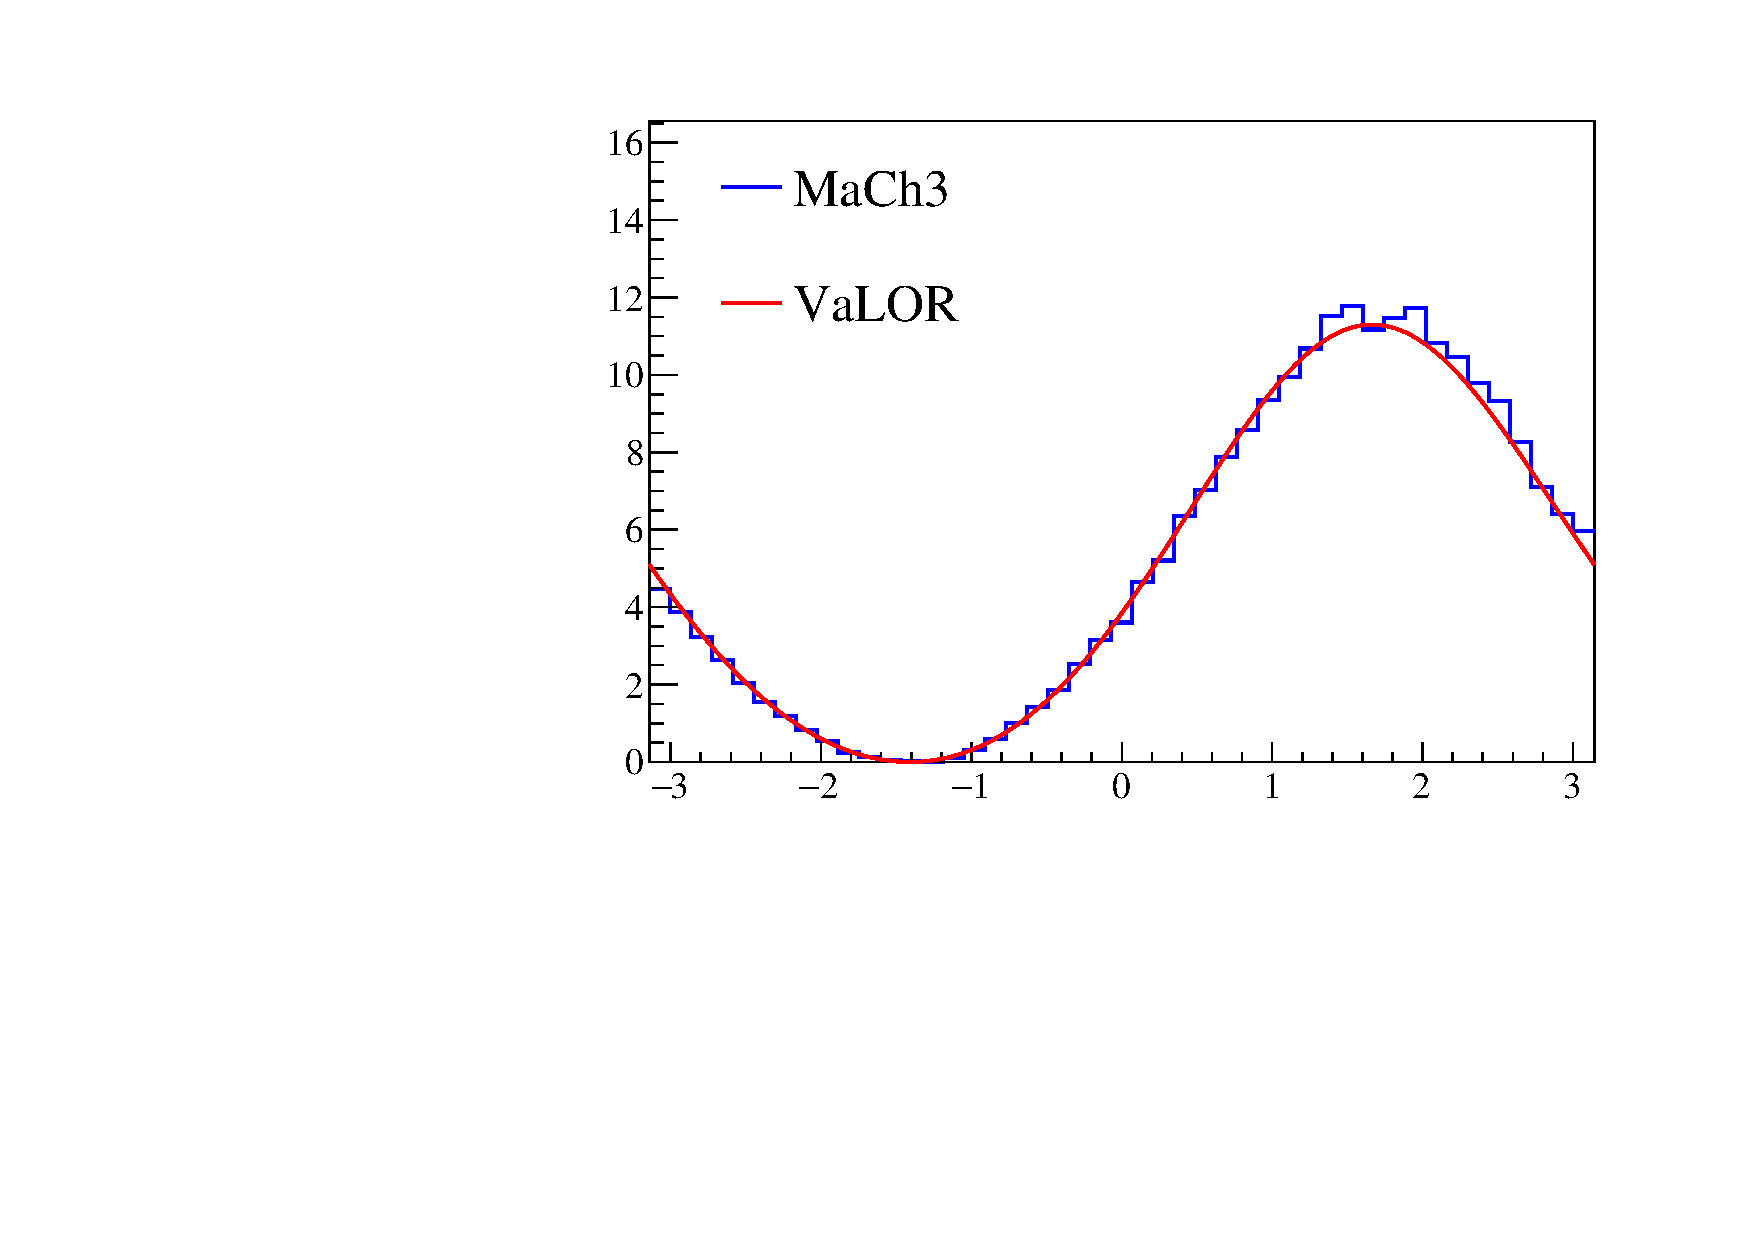
\includegraphics[width=\textwidth]{TalkPics/2Ddatafit_270916/comparedcontours_2D_mach3valor_wRC_dcp_IH.pdf}
    \end{columns}
  \end{frame}

  \begin{frame}
    \frametitle{}
    \label{lastframe}
    \begin{block}{}
      \begin{itemize}
      \item Fairly good agreement seen between MaCh3 and Valor when MaCh3 move to the same binning for $\nu_{e}$
      \item Confirms that tighter constraint seen by Valor for Run 1-7c is due to binning
      \item[-] Previously seen that 1D binned Valor analysis gave same result as 1D MaCh3
      \item We plan to use 2D binning for $\nu_{e}$ for future MaCh3 analyses and will look into 2D binning for $\nu_{\mu}$ as well
      \end{itemize}
    \end{block}
  \end{frame}

  %Backup goes here
  \begin{frame}
    \centering
    \huge\textcolor{beamer@icmiddleblue}{MaCh3 1D-2D Asimov comparisons woRC}
  \end{frame}

  \begin{frame}
    \centering
    \begin{columns}
      \column{.6\textwidth}
      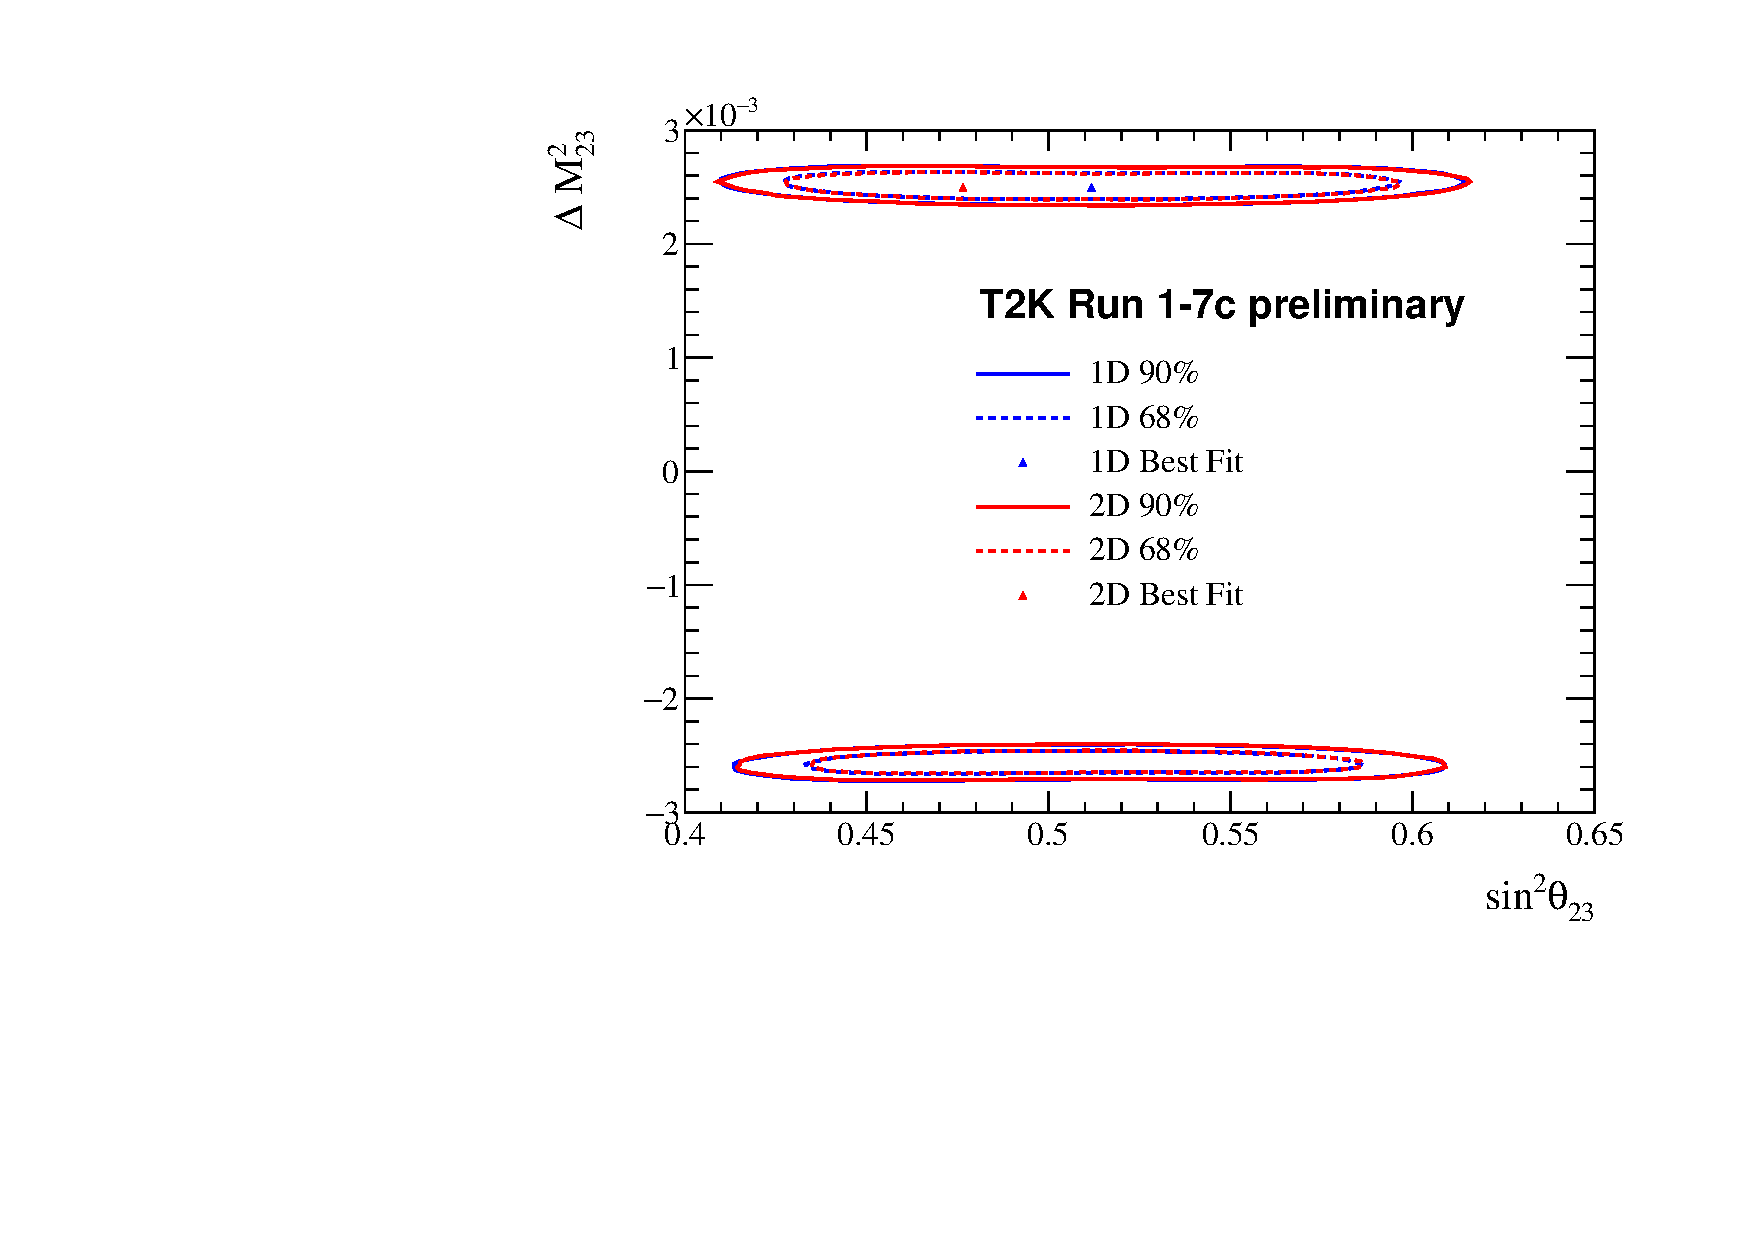
\includegraphics[width=\textwidth]{TalkPics/2Ddatafit_270916/contours_1D2Dasimovcomparisons_woRC/comparedcontours_th23dm23_1Dvs2D_official.pdf}
      \column{.6\textwidth}
      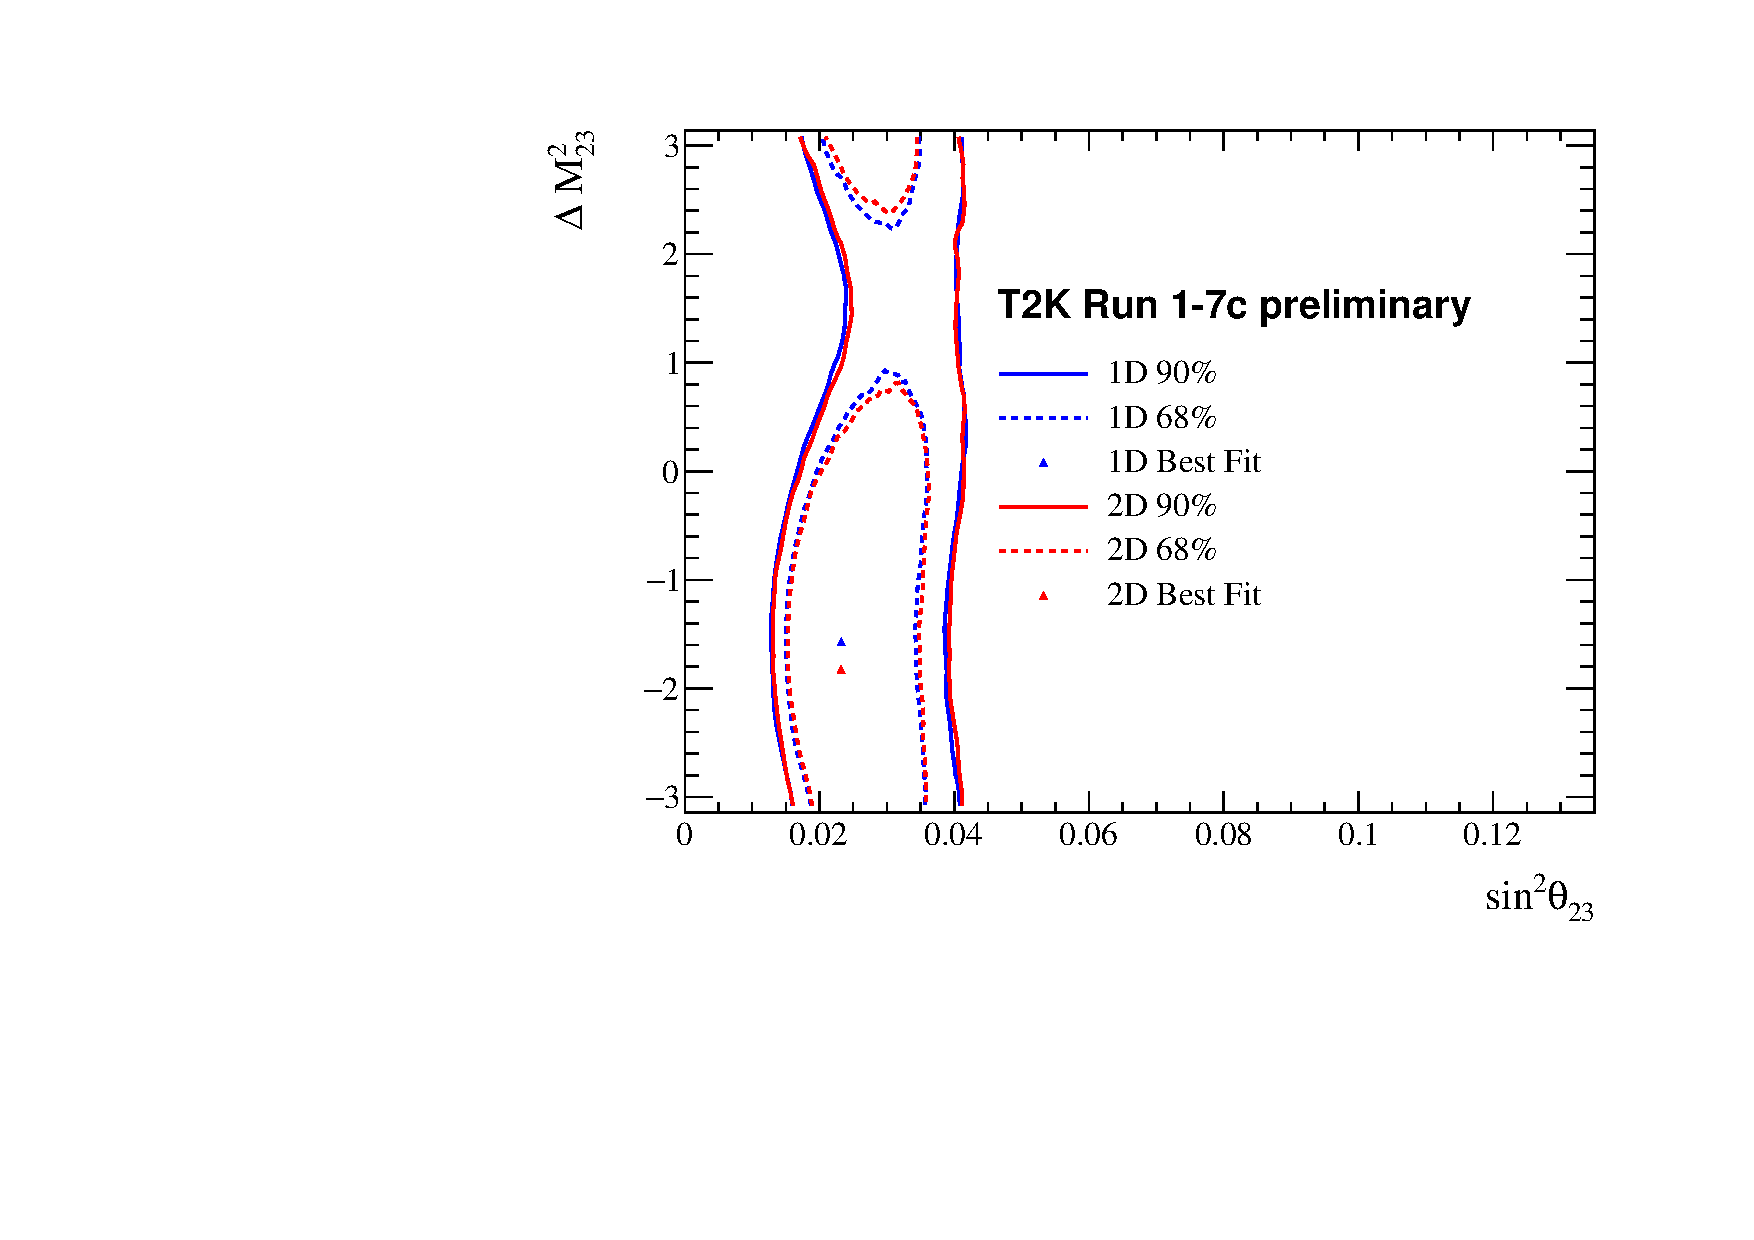
\includegraphics[width=\textwidth]{TalkPics/2Ddatafit_270916/contours_1D2Dasimovcomparisons_woRC/comparedcontours_th13dcp_1Dvs2D_official.pdf}
    \end{columns}
  \end{frame}

  \begin{frame}
    \centering
    \begin{columns}
      \column{.6\textwidth}
      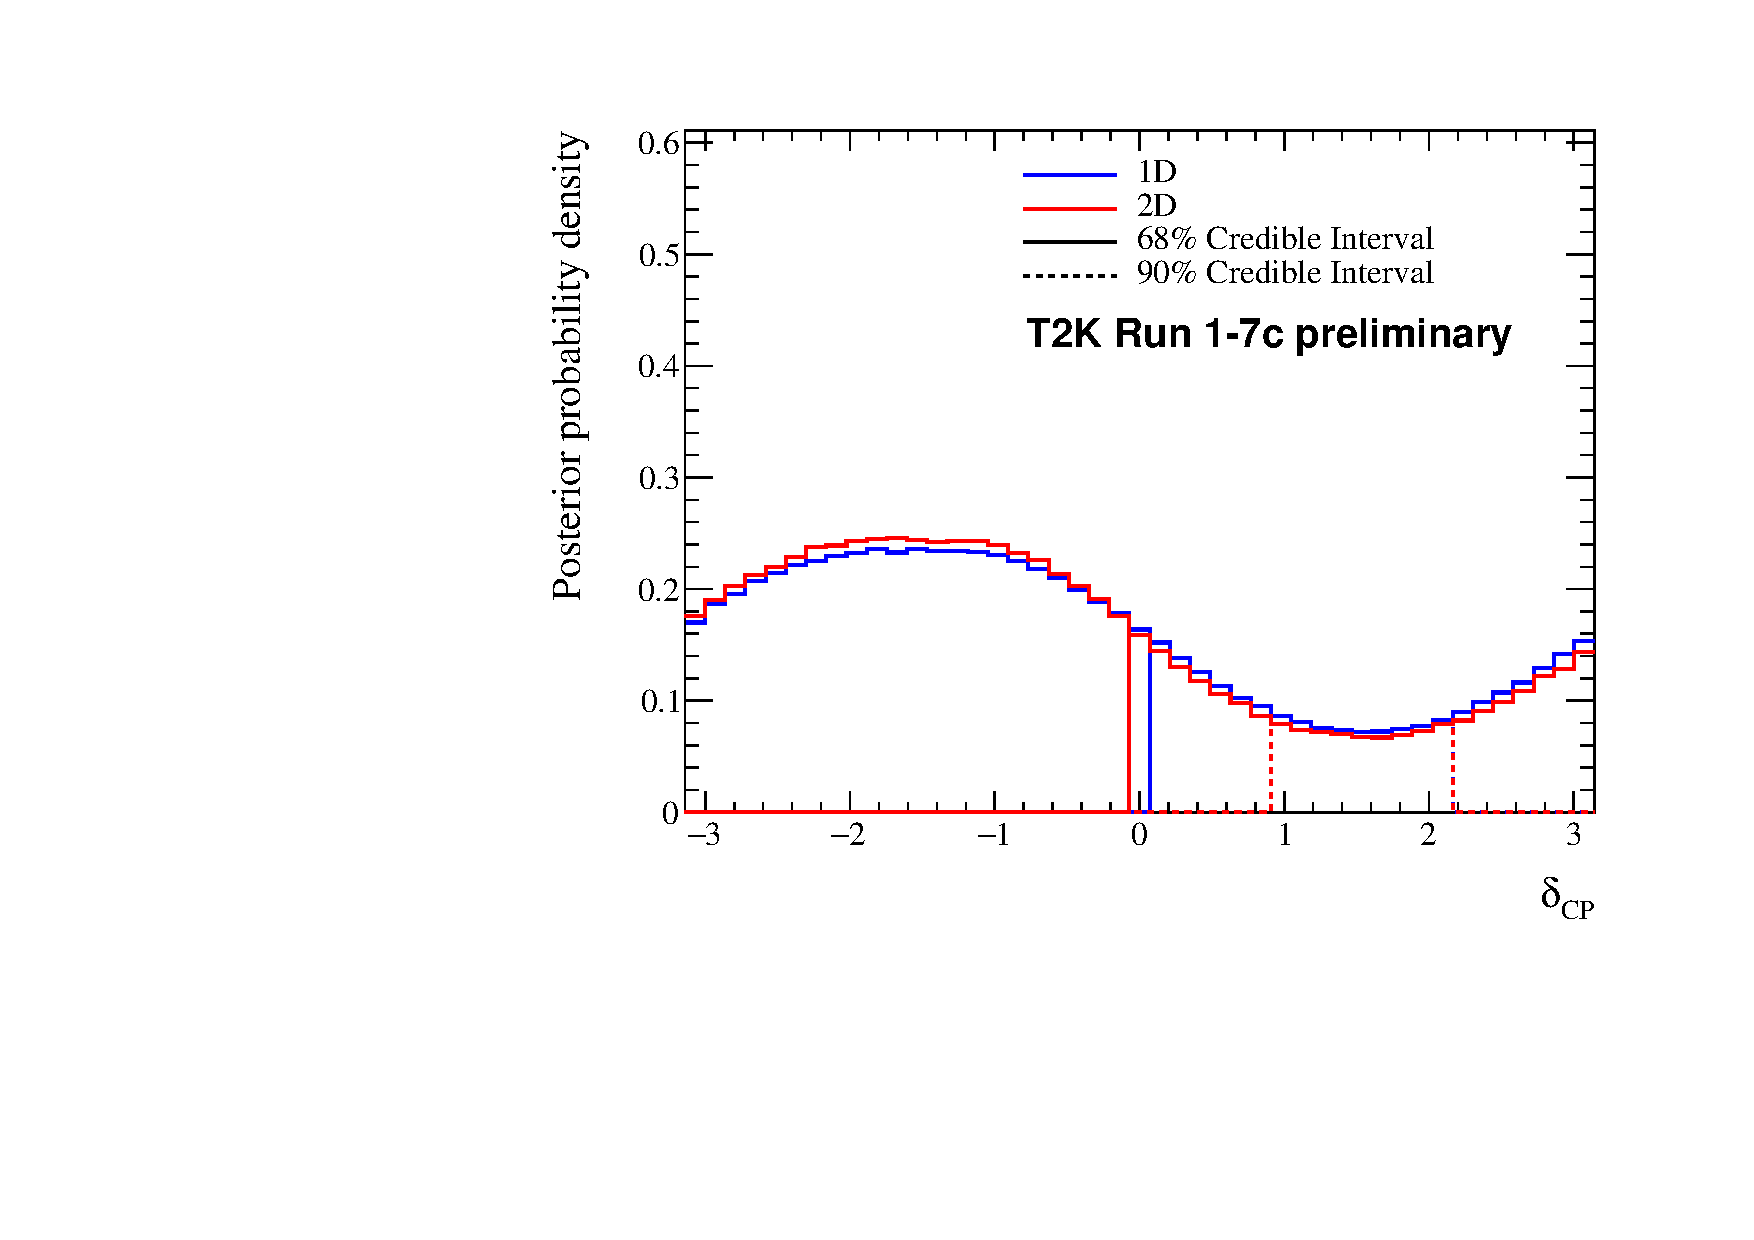
\includegraphics[width=\textwidth]{TalkPics/2Ddatafit_270916/contours_1D2Dasimovcomparisons_woRC/contours_1D_dcp_compare_official.pdf}
    \end{columns}
  \end{frame}

  
\end{fmffile}
\end{document}

